% 'draft' mode can be used to speed up compilation
\documentclass[twoside,final]{hcmut-report}
\usepackage{codespace}

% Encodings & symbols
\usepackage{gensymb,textcomp}

% Better tables
\usepackage{array,longtable,multicol,multirow,siunitx,tabularx}

% Better lists
\usepackage{enumitem}

% Graphics
\usepackage{caption,float}
\usepackage[export]{adjustbox}

% Cross-references (use \Cref{} instead of \ref{})
\usepackage[nameinlink]{cleveref}

% Graphics search paths
\graphicspath{{graphics/}{figures/}}

% --- Metadata ---
\coursename{\parbox[c]{0.85\linewidth}{\centering CO5177 -- Nền tảng lập trình cho phân tích và trực quan dữ liệu}}
\reporttype{Báo cáo Bài tập lớn (Group6)}
\title{Phân tích, Trực quan hóa và Mô hình hóa Dữ liệu Đa dạng thức (Tabular, Text, Image)}
\advisor{& TS. Lê Thành Sách &}
\stuname{%
  & Lê Đình Đức & 2310774 \\
  & Nguyễn Văn Công Thành & 2313133 \\
}

\AtBeginDocument{\counterwithin{lstlisting}{section}}

\begin{document}
\coverpage%

\section*{Thông tin nhóm và Phân công công việc}
\begin{itemize}[leftmargin=*]
  \item \textbf{Tên nhóm:} Group6 (CH01 -- Học kỳ 261, Năm học 2026--2027)
  \item \textbf{Kho mã nguồn:} \href{https://github.com/dducsw/co5177-data-analytics-and-visualization-project}{\texttt{github.com/dducsw/co5177-data-analytics-and-visualization-project}}
\end{itemize}

\newcounter{memberrowno}
\setcounter{memberrowno}{0}
\begin{center}
  \begin{tabularx}{\linewidth}{>{\stepcounter{memberrowno}\thememberrowno}c l c X c}
    \toprule
    \multicolumn{1}{c}{\textbf{STT}} & \textbf{Họ và tên} & \textbf{MSSV} & \textbf{Vai trò \& Đóng góp chính} & \textbf{Tỷ lệ} \\
    \midrule
    & Lê Đình Đức & 2310774 & Thu thập dữ liệu, EDA, xây dựng pipeline mô hình, trực quan hóa kết quả và hoàn thiện báo cáo & 100\% \\
    & Nguyễn Văn Công Thành & 2313133 & Thiết kế thực nghiệm đối chứng, kiểm chứng giả thuyết, phân tích lỗi và hoàn thiện báo cáo & 100\% \\
    \bottomrule
  \end{tabularx}
\end{center}
\clearpage

\tableofcontents
\listoffigures
\listoftables

\clearpage
\section{Giới thiệu chung}
\label{sec:intro}

Trong thực hành khoa học dữ liệu hiện đại, mỗi dạng dữ liệu đặt ra những thách thức riêng về chất lượng mẫu, nguy cơ rò rỉ thông tin (\textit{data leakage}) và tiêu chí đánh giá mô hình. Dữ liệu bảng trong lĩnh vực tài chính thường mất cân bằng nghiêm trọng và biến đổi theo thời gian; dữ liệu văn bản báo chí tiếng Việt lại vướng vấn đề chuẩn hóa dấu thanh, phân đoạn từ ghép và các bản tin định kỳ gần giống nhau; trong khi dữ liệu ảnh đòi hỏi cân nhắc kỹ giữa độ chính xác phân loại, chi phí tài nguyên và khả năng giải thích quyết định của mạng nơ-ron sâu.

Báo cáo này trình bày kết quả nghiên cứu, trực quan hóa và thực nghiệm mô hình trên ba bài toán đại diện cho ba dạng dữ liệu trên: (1) phát hiện gian lận mở tài khoản ngân hàng trên tập dữ liệu bảng \textit{Bank Account Fraud}, (2) phân loại tin tức kinh tế -- tài chính tiếng Việt thu thập từ báo điện tử \textit{VnEconomy}, và (3) phân loại ảnh cảnh quan tự nhiên trên bộ \textit{Intel Image Classification}. Thay vì dừng ở việc huấn luyện một mô hình đơn lẻ, toàn bộ thực nghiệm được triển khai theo một nguyên tắc xuyên suốt: đặt câu hỏi định lượng ngay từ bước khám phá dữ liệu (\textit{EDA}), thiết kế phép chia tập và quy trình tiền xử lý phù hợp với bối cảnh vận hành thực tế, sau đó đối chiếu nhiều họ mô hình kèm kiểm định thống kê và phân tích lỗi.

\begin{table}[H]
  \centering
  \caption{Tóm tắt ba bài toán, quy mô dữ liệu và trọng tâm phương pháp luận.}
  \label{tab:overview_datasets}
  \begin{tabularx}{\linewidth}{l p{3.1cm} p{3.1cm} X}
    \toprule
    \textbf{Dạng dữ liệu} & \textbf{Tập dữ liệu} & \textbf{Quy mô} & \textbf{Thách thức \& Phương pháp chính} \\
    \midrule
    Bảng (\textit{Tabular}) & Bank Account Fraud (\texttt{Base.csv}) \cite{jesus2022turning} & 1.000.000 hồ sơ, 32 thuộc tính, 2 lớp & Tỷ lệ gian lận 1,10\%, dữ liệu khuyết mã hóa bằng số âm và dịch chuyển phân phối theo thời gian. Dùng \textit{Temporal Split}, đối chiếu Logistic Regression với LightGBM, đánh giá Bootstrap và công bằng theo nhóm tuổi. \\
    Văn bản (\textit{Text}) & Tin tức tài chính VnEconomy (tự thu thập) & 5.000 bài báo, 11 trường, 5 chuyên mục & Chuẩn hóa Unicode/dấu thanh tiếng Việt, cụm bài gần trùng (5,0\%) và rò rỉ theo tác giả. Dùng \textit{StratifiedGroupKFold}, TF-IDF, đối chiếu MultinomialNB, Logistic Regression và LinearSVC. \\
    Ảnh (\textit{Image}) & Intel Image Classification \cite{bansal2019intel} & 17.034 ảnh RGB (14.034 Train, 3.000 Test), 6 lớp & Giao thoa thị giác giữa các cặp cảnh quan gần giống nhau. Đối chiếu 7 cấu hình thuộc 4 hướng: \textit{From Scratch}, \textit{Linear Probe}, \textit{Fine-tuning} (ResNet-18, ViT-B/16), \textit{Zero-shot CLIP} và Grad-CAM. \\
    \bottomrule
  \end{tabularx}
\end{table}

Cấu trúc các phần tiếp theo được tổ chức tương ứng với từng bài toán: \Cref{sec:tabular} đi sâu vào bài toán dữ liệu bảng, \Cref{sec:text} phân tích ngữ liệu văn bản tiếng Việt, \Cref{sec:image} trình bày chuỗi thực nghiệm phân loại ảnh, và \Cref{sec:conclusion} tổng kết các nhận định kỹ thuật cùng giới hạn khách quan của nghiên cứu.

\section{Dữ liệu bảng: Phát hiện gian lận mở tài khoản ngân hàng}
\label{sec:tabular}

\subsection{Bối cảnh bài toán, toàn vẹn dữ liệu và phân chia theo thời gian}
Trong nghiệp vụ mở tài khoản ngân hàng trực tuyến, gian lận thường diễn ra dưới hình thức mạo danh hoặc tạo lập danh tính giả nhằm chiếm đoạt hạn mức tín dụng đi kèm. Hệ quả của sai số phân loại có tính bất đối xứng rõ rệt: bỏ sót hồ sơ gian lận gây tổn thất tài chính trực tiếp cho ngân hàng, trong khi chặn nhầm hồ sơ hợp pháp lại từ chối quyền tiếp cận dịch vụ tài chính cơ bản của khách hàng. Thực nghiệm trong chương này sử dụng tập dữ liệu chuẩn \texttt{Base.csv} thuộc bộ \textit{Bank Account Fraud (BAF)} \cite{jesus2022turning}, được tổng hợp bằng CTGAN từ dữ liệu ngân hàng thực đã ẩn danh, gồm \textbf{1.000.000 hồ sơ} trải dài qua 8 tháng (mã hóa \texttt{month} từ 0 đến 7) với \textbf{32 thuộc tính} (18 cột nguyên, 9 cột thực, 5 cột phân loại) và không có bản ghi trùng lặp hoàn toàn.

Kiểm tra bước đầu cho thấy ba đặc điểm cần xử lý trước khi phân tích sâu. Thứ nhất, biến mục tiêu \texttt{fraud\_bool} mất cân bằng nặng (\Cref{fig:tab_dist_shift}, bên trái): chỉ có 11.029 hồ sơ gian lận (1,10\%) so với 988.971 hồ sơ hợp pháp (98,90\%), tức xấp xỉ 1 ca gian lận trên 89 hồ sơ. Với tỷ lệ này, thước đo \textit{Accuracy} trở nên vô nghĩa vì một bộ phân loại luôn dự đoán hợp pháp đã đạt 98,90\% nhưng bỏ lọt toàn bộ gian lận. Do đó, thước đo chính được áp dụng theo \cite{jesus2022turning} là \textbf{TPR@5\%FPR} (tỷ lệ phát hiện gian lận khi khống chế tỷ lệ báo động nhầm đối với khách hàng hợp pháp không vượt quá 5\%), đi kèm \textit{ROC-AUC}, \textit{PR-AUC} và ma trận nhầm lẫn.

Thứ hai, dù Pandas ghi nhận 0 giá trị \texttt{NaN} mặc định, đối chiếu với tài liệu đặc tả dữ liệu cho thấy cột \texttt{device\_fraud\_count} chỉ mang một giá trị hằng số duy nhất là \texttt{0} nên được loại bỏ, đồng thời 6 cột thực chất mã hóa dữ liệu khuyết bằng số âm: giá trị \texttt{-1} ở \texttt{prev\_address\_months\_count} (712.920 dòng), \texttt{bank\_months\_count} (253.635 dòng), \texttt{current\_address\_months\_count} (4.254 dòng), \texttt{session\_length\_in\_minutes} (2.015 dòng), \texttt{device\_distinct\_emails\_8w} (359 dòng) và mọi giá trị âm ($< 0$) ở \texttt{intended\_balcon\_amount} (742.523 dòng, chiếm 74,25\%). Riêng 488 dòng mang giá trị \texttt{-1} ở \texttt{credit\_risk\_score} nằm trong miền điểm hợp lệ $[-191, 389]$ nên được giữ nguyên. Với 6 cột khuyết ẩn này, giá trị khuyết được chuẩn hóa về \texttt{NaN} sau khi tạo tương ứng 6 cột cờ nhị phân \texttt{\_flag} nhằm bảo lưu tín hiệu hành vi không khai báo thông tin.

Thứ ba, tỷ lệ gian lận không dừng theo thời gian (\Cref{fig:tab_dist_shift}, bên phải): dao động trong khoảng 0,875\%--1,183\% từ tháng 0 đến tháng 5, rồi tăng lên 1,341\% ở tháng 6 và 1,475\% ở tháng 7, trong khi lượng hồ sơ giảm dần từ 150.936 (tháng 3) xuống 96.843 (tháng 7). Sự hiện diện của \textit{temporal shift} khiến phép chia ngẫu nhiên (trộn lẫn các tháng) tạo ra rò rỉ thông tin tương lai (\textit{look-ahead bias}). Vì vậy, dữ liệu được tách nghiêm ngặt theo trục thời gian (\textit{Temporal Split}, \Cref{tab:tab_split}); mọi khảo sát EDA, tính toán thống kê và khớp bộ tiền xử lý từ đây trở đi chỉ tiến hành trên tập Train.

\begin{figure}[H]
  \centering
  \begin{minipage}[b]{0.47\linewidth}
    \centering
    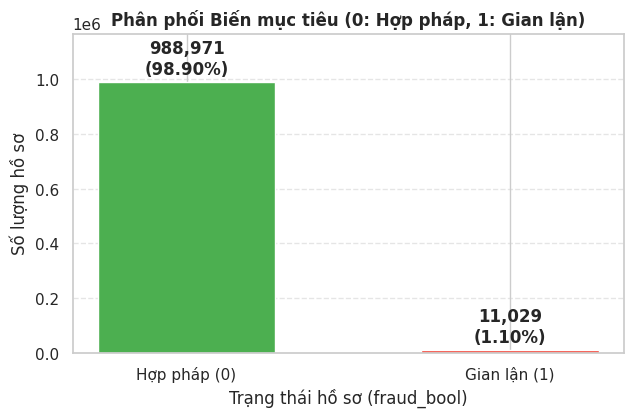
\includegraphics[width=\linewidth]{tabular/c13_f0.png}
  \end{minipage}\hfill
  \begin{minipage}[b]{0.51\linewidth}
    \centering
    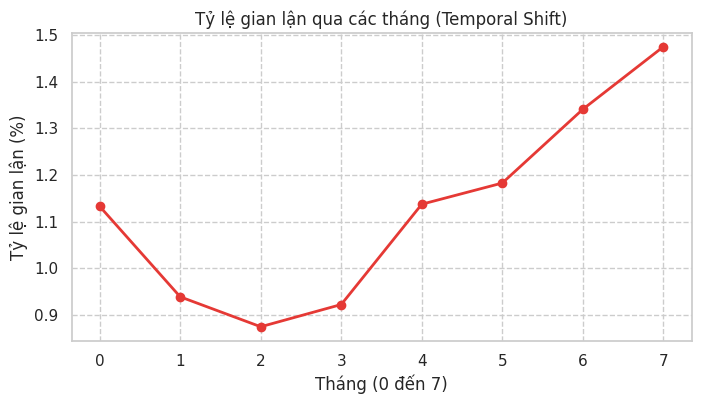
\includegraphics[width=\linewidth]{tabular/c25_f0.png}
  \end{minipage}
  \caption{Phân phối biến mục tiêu \texttt{fraud\_bool} (trái) và biến động tỷ lệ gian lận qua 8 tháng (phải) trên toàn tập \texttt{Base.csv}.}
  \label{fig:tab_dist_shift}
\end{figure}

\begin{table}[H]
  \centering
  \caption{Cấu trúc phân chia theo thời gian (\textit{Temporal Split}) của tập \texttt{Base.csv}.}
  \label{tab:tab_split}
  \resizebox{\linewidth}{!}{%
  \begin{tabular}{l c r r c c}
    \toprule
    \textbf{Tập dữ liệu} & \textbf{Tháng} & \textbf{Số hồ sơ} & \textbf{Số ca gian lận} & \textbf{Tỷ trọng (\%)} & \textbf{Tỷ lệ gian lận (\%)} \\
    \midrule
    Train & 0 -- 5 & 794.989 & 8.151 & 79,50 & 1,03 \\
    Validation & 6 & 108.168 & 1.450 & 10,82 & 1,34 \\
    Test & 7 & 96.843 & 1.428 & 9,68 & 1,47 \\
    \bottomrule
  \end{tabular}%
  }
\end{table}

\subsection{Khám phá dữ liệu trên tập huấn luyện}

\subsubsection{Cơ chế dữ liệu khuyết và ảnh hưởng của việc điền trung vị}
Để kiểm tra việc bỏ trống thông tin là ngẫu nhiên (\textit{MCAR}) hay gắn với hành vi rủi ro (\textit{MNAR}), tỷ lệ gian lận được đối chiếu giữa nhóm thiếu (\texttt{flag = 1}) và nhóm khai báo đủ (\texttt{flag = 0}) thông qua tỷ số rủi ro (\textit{Risk Ratio}) trên \texttt{df\_train}. Kết quả ở \Cref{fig:tab_missing} cho thấy dữ liệu khuyết mang tín hiệu phân tách mạnh ở ba cột thiếu nhiều nhất: với \texttt{prev\_address\_months\_count} (thiếu 71,50\%), nhóm không khai báo có tỷ lệ gian lận 1,32\% so với chỉ 0,28\% ở nhóm có khai báo địa chỉ cũ (chênh lệch \textbf{4,73 lần}); tương tự, rủi ro tăng \textbf{2,58 lần} khi thiếu \texttt{intended\_balcon\_amount} (1,22\% vs 0,47\%) và \textbf{1,80 lần} khi thiếu \texttt{bank\_months\_count} (1,54\% vs 0,85\%). Ba cột còn lại thiếu dưới 0,4\% và có tỷ số rủi ro gần trung tính.

\begin{figure}[H]
  \centering
  \begin{minipage}[b]{0.55\linewidth}
    \centering
    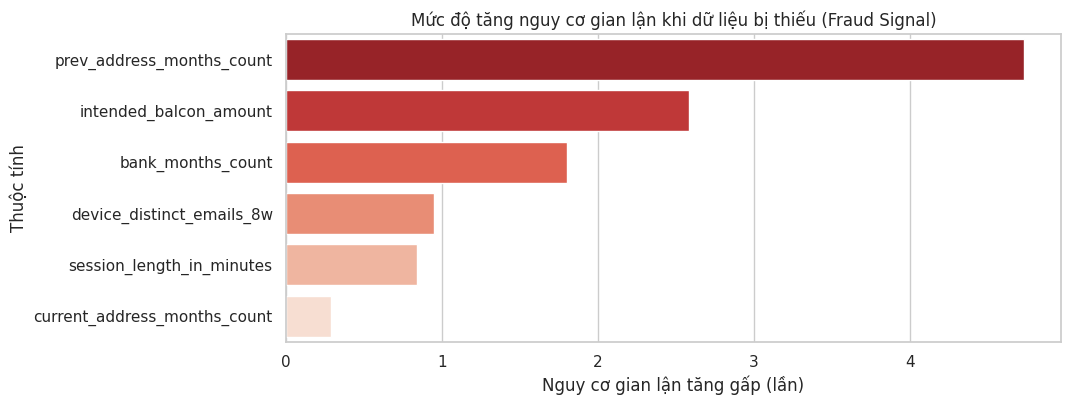
\includegraphics[width=\linewidth]{tabular/c31_f0.png}
  \end{minipage}\hfill
  \begin{minipage}[b]{0.43\linewidth}
    \centering
    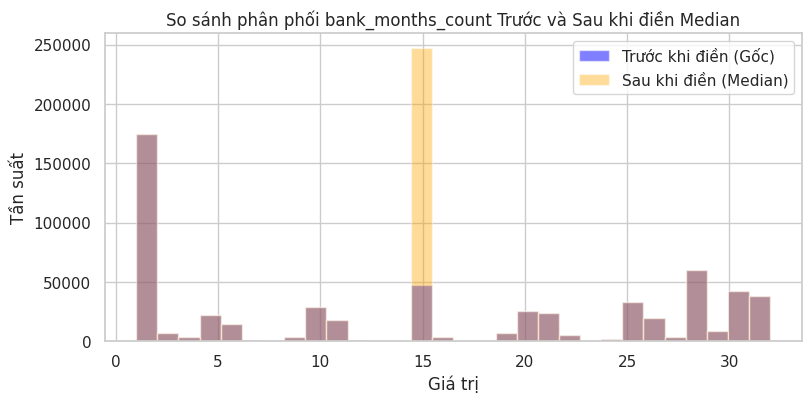
\includegraphics[width=\linewidth]{tabular/c33_f0.png}
  \end{minipage}
  \caption{Tỷ số tăng nguy cơ gian lận khi khuyết dữ liệu (trái) và biến dạng phân phối của \texttt{bank\_months\_count} khi điền trung vị bằng 15 tháng (phải).}
  \label{fig:tab_missing}
\end{figure}

Thử nghiệm điền khuyết bằng trung vị (\textit{median} = 15,0 tháng) trên \texttt{bank\_months\_count} (\Cref{fig:tab_missing}, bên phải) tạo ra một đỉnh nhọn nhân tạo chiếm 25,10\% mẫu, làm méo phân phối thực và trộn lẫn nhóm bỏ trống với nhóm có thâm niên tài khoản 15 tháng. Do đó, tập dữ liệu được giữ nguyên giá trị \texttt{NaN} kết hợp 6 cờ \texttt{\_flag} cho mô hình cây; phép điền trung vị chỉ áp dụng nội bộ trong pipeline của mô hình tuyến tính.

\subsubsection{Phân hóa rủi ro theo biến phân loại, kênh nộp đơn và hành vi phiên}
Khảo sát nhóm biến phân loại và cờ định danh trên \texttt{df\_train} (\Cref{fig:tab_cat_flags}) ghi nhận sự phân hóa rõ rệt quanh mức nền 1,03\%. Ở biến hệ điều hành (\texttt{device\_os}), nhóm \texttt{windows} (26,8\% hồ sơ) có tỷ lệ gian lận 2,30\%, cao hơn gấp đôi mức nền, theo sau là \texttt{macintosh} (1,26\%), trong khi \texttt{linux} và \texttt{other} ở quanh mức 0,5\%. Với phương thức thanh toán (\texttt{payment\_type}), nhóm \texttt{AC} dẫn đầu ở mức 1,58\%, còn ở tình trạng nhà ở (\texttt{housing\_status}), nhóm \texttt{BA} ghi nhận tỷ lệ rủi ro nổi bật nhất so với các nhóm còn lại.

\begin{figure}[H]
  \centering
  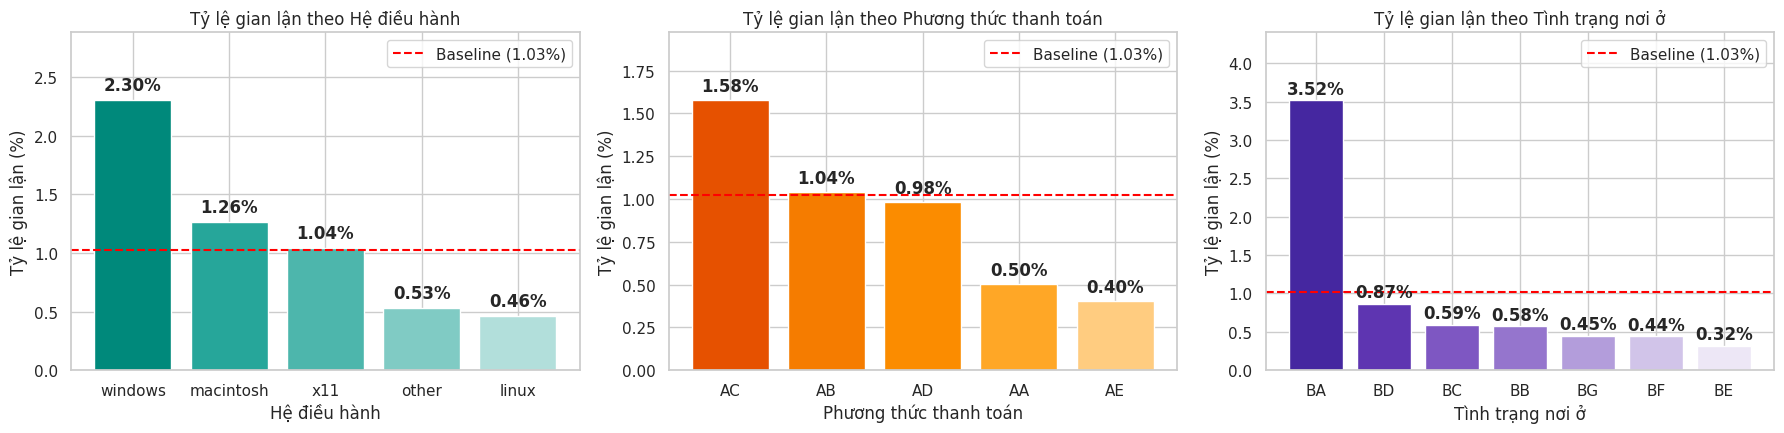
\includegraphics[width=0.96\linewidth]{tabular/c36_f0.png}\\[4pt]
  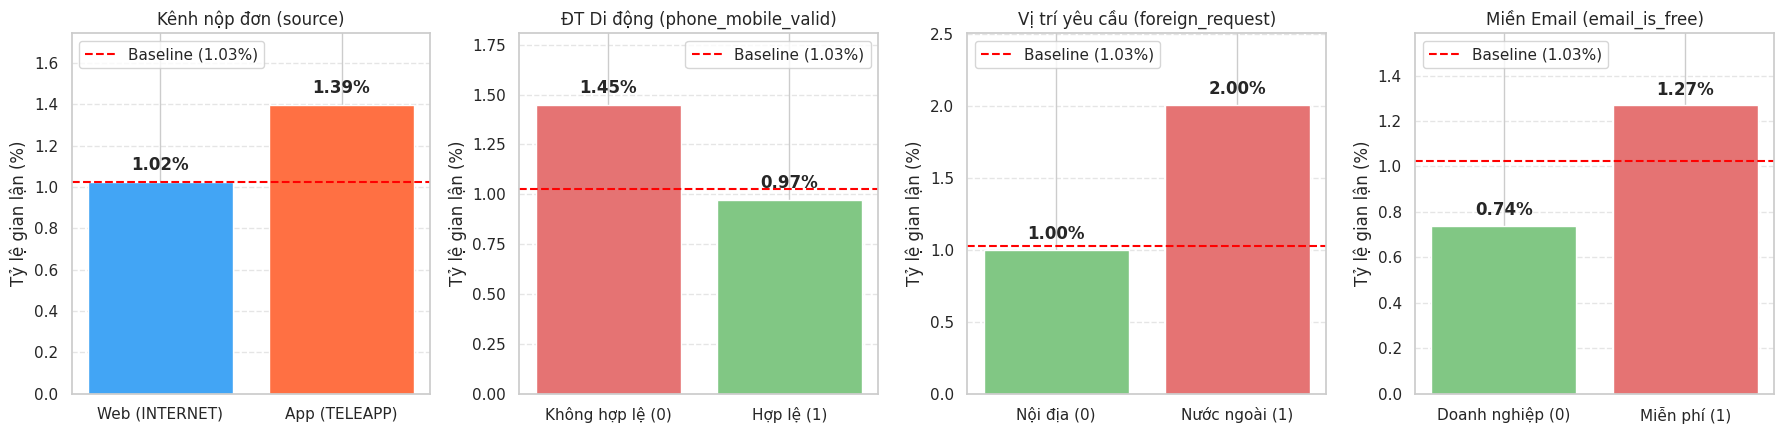
\includegraphics[width=0.96\linewidth]{tabular/c38_f0.png}\\[4pt]
  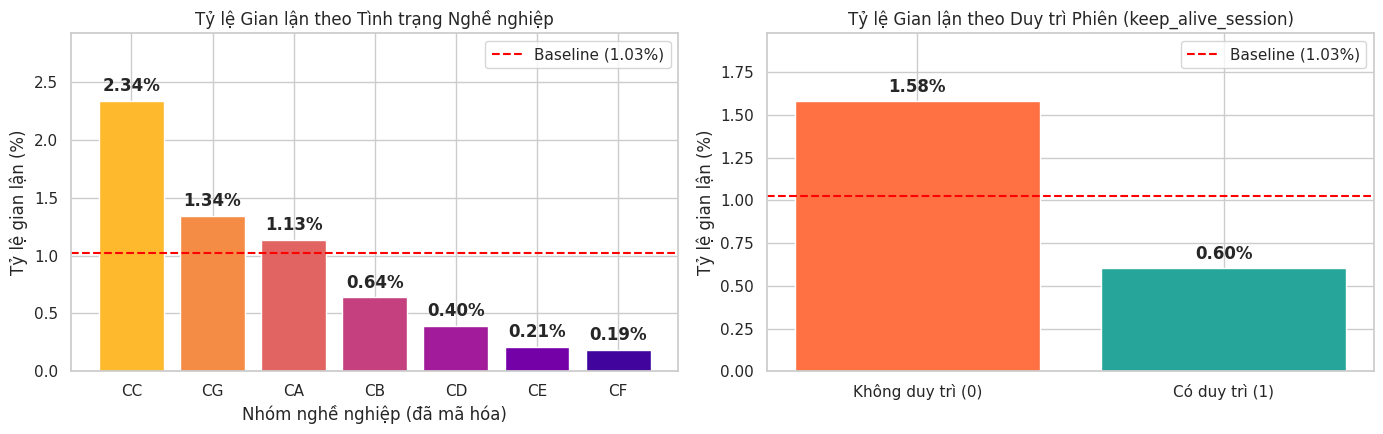
\includegraphics[width=0.80\linewidth]{tabular/c40_f0.png}
  \caption{Tỷ lệ gian lận trên tập huấn luyện phân theo các biến phân loại chính (trên), nhóm cờ định danh -- kênh nộp đơn (giữa), tình trạng nghề nghiệp và duy trì phiên (dưới).}
  \label{fig:tab_cat_flags}
\end{figure}

Xét các cờ xác thực và hành vi phiên, yêu cầu xuất phát từ nước ngoài (\texttt{foreign\_request = 1}) có tỷ lệ gian lận 2,00\% so với 1,00\% nội địa; hồ sơ không duy trì phiên (\texttt{keep\_alive\_session = 0}) có rủi ro 1,58\% so với 0,60\% khi duy trì; số điện thoại di động hoặc cố định không hợp lệ (\texttt{phone\_mobile\_valid = 0}: 1,45\%; \texttt{phone\_home\_valid = 0}: 1,29\%) và email miễn phí (\texttt{email\_is\_free = 1}: 1,27\% vs 0,74\%) đều gắn với mức rủi ro cao hơn. Kênh ứng dụng di động (\texttt{TELEAPP}) tuy chỉ chiếm 5.737 đơn nhưng có tỷ lệ gian lận 1,39\% so với 1,02\% của kênh web (\texttt{INTERNET}). Đáng chú ý, tình trạng nghề nghiệp (\texttt{employment\_status}) phân hóa tới hơn 12 lần, từ 2,34\% ở nhóm \texttt{CC} xuống còn 0,19\% ở nhóm \texttt{CF}.

\subsubsection{Biến vận tốc, giá trị ngoại lai và tín hiệu thiết bị}
Một giả thuyết phổ biến trong phòng chống gian lận là tốc độ nộp đơn quá cao (\texttt{velocity\_6h}) thường phản ánh tấn công tự động. Tuy nhiên, kiểm tra bằng quy tắc IQR (ngưỡng trên 14.326,7 đơn/giờ, chiếm 6.498 hồ sơ hay 0,82\%) và phân tầng theo thập phân vị (\Cref{fig:tab_velocity}) lại cho kết quả ngược chiều: nhóm ngoại lai chỉ có tỷ lệ gian lận 0,65\% (thấp hơn mức nền 1,03\%), và tỷ lệ gian lận giảm gần như đơn điệu từ 1,34\% ở thập phân vị thấp nhất (D1) xuống 0,70\% ở thập phân vị cao nhất (D10). Do ngoại lai không phải là nhiễu đo lường hay cụm gian lận riêng biệt, toàn bộ các điểm cực trị (kể cả 20 hồ sơ có \texttt{velocity\_6h < 0}) đều được giữ lại thay vì cắt bỏ.

\begin{figure}[H]
  \centering
  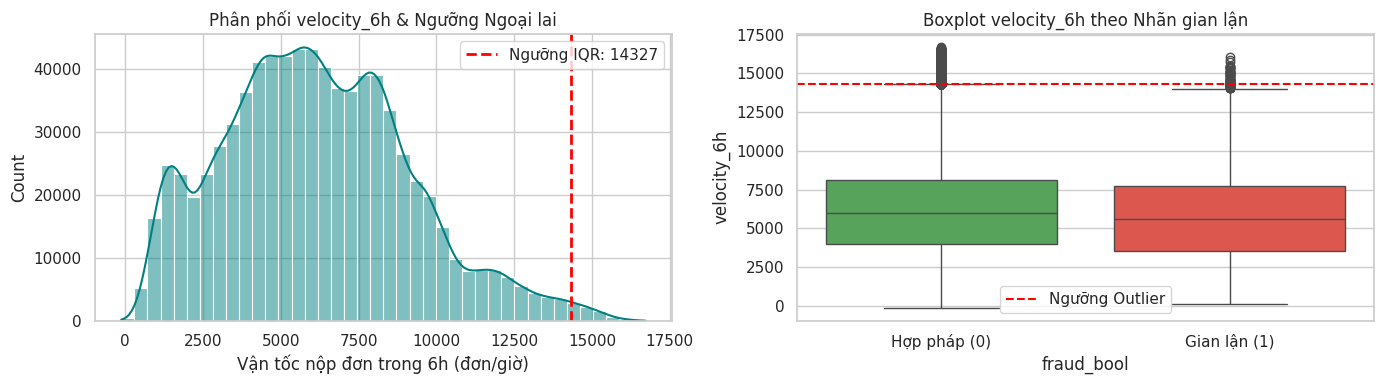
\includegraphics[width=0.92\linewidth]{tabular/c42_f0.png}\\[4pt]
  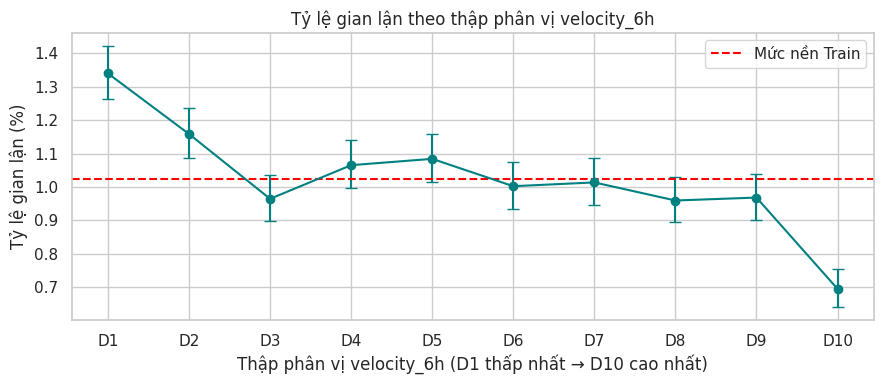
\includegraphics[width=0.68\linewidth]{tabular/c42_f1.png}
  \caption{Phân phối, ngưỡng ngoại lai IQR của \texttt{velocity\_6h} (trên) và tỷ lệ gian lận giảm dần theo 10 thập phân vị vận tốc (dưới).}
  \label{fig:tab_velocity}
\end{figure}

Ba khung vận tốc (\texttt{velocity\_6h}, \texttt{velocity\_24h}, \texttt{velocity\_4w}) chỉ có tương quan tuyến tính ở mức trung bình ($r \in [0,30; 0,40]$), bổ trợ thông tin cho nhau mà không gây đa cộng tuyến nghiêm trọng. Với các biến hành vi và thiết bị khác (\Cref{fig:tab_behavior}), độ trễ nộp đơn \texttt{days\_since\_request} từ 1 đến 5 ngày ghi nhận rủi ro 1,99\% (gấp đôi nhóm nộp ngay trong ngày là 1,01\%); hồ sơ phát sinh tại chi nhánh không có lưu lượng trong 8 tuần (\texttt{bank\_branch\_count\_8w = 0}) đạt 1,68\% so với 0,72\% ở chi nhánh có trên 100 đơn; và phiên thao tác kéo dài trên 30 phút đạt 1,80\% so với mức 0,98\%--1,05\% của phiên 2--15 phút. Đặc biệt, khi một thiết bị được sử dụng với 2 địa chỉ email khác nhau trong 8 tuần (\texttt{device\_distinct\_emails\_8w = 2}, 22.583 đơn), tỷ lệ gian lận tăng lên \textbf{3,88\%}, gấp gần 4 lần mức nền; ngược lại, \texttt{date\_of\_birth\_distinct\_emails\_4w} có xu hướng giảm rủi ro khi số email tăng (từ 1,81\% ở nhóm $\le 5$ về 0,61\%, $r = -0,043$).

\begin{figure}[H]
  \centering
  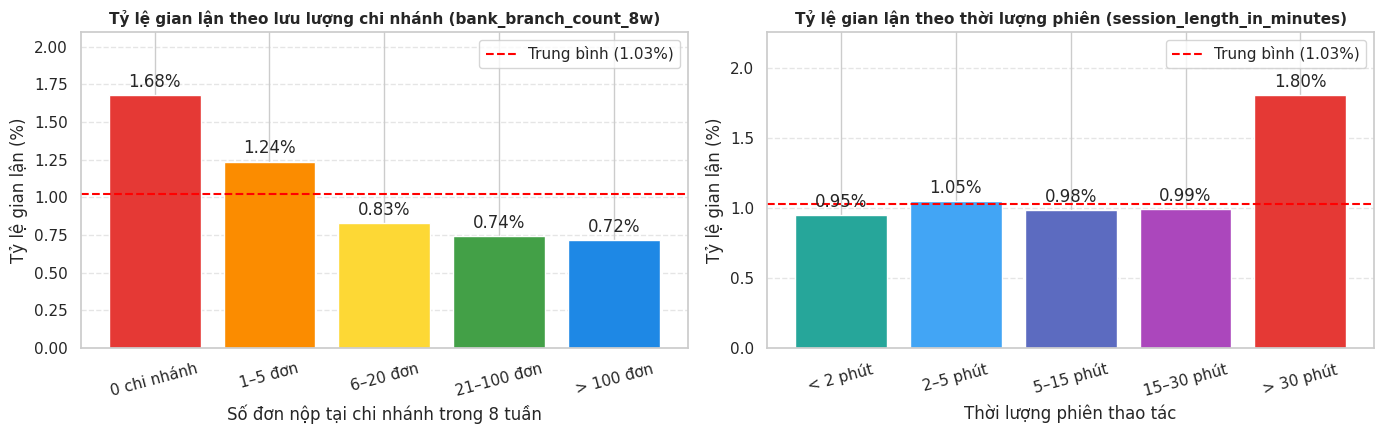
\includegraphics[width=0.88\linewidth]{tabular/c46_f0.png}\\[4pt]
  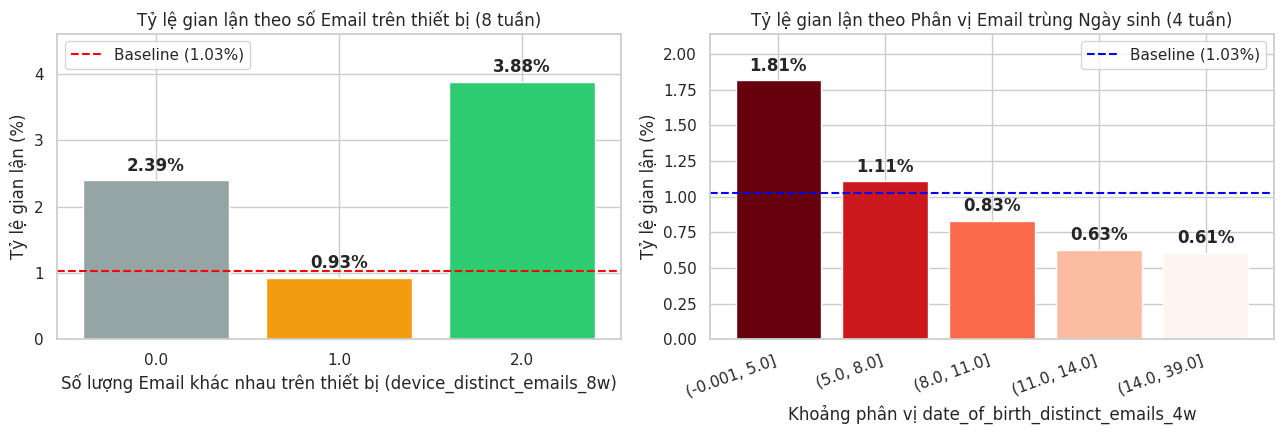
\includegraphics[width=0.88\linewidth]{tabular/c48_f0.png}
  \caption{Tỷ lệ gian lận theo lưu lượng chi nhánh, thời lượng phiên (trên) và theo số email dùng chung thiết bị, ngày sinh (dưới).}
  \label{fig:tab_behavior}
\end{figure}

\subsubsection{Đặc trưng tài chính, tương tác phi tuyến và độ ổn định phân phối}
Ở nhóm biến tài chính, hạn mức tín dụng do ứng viên tự đề xuất (\texttt{proposed\_credit\_limit}) tỷ lệ thuận với rủi ro: tăng từ 0,68\% (mức $\le 200$) lên 0,96\% (201--500) và 1,90\% ($> 500$). Ngược lại, việc đã sở hữu thẻ khác tại cùng ngân hàng (\texttt{has\_other\_cards = 1}) đóng vai trò tín hiệu an toàn rõ rệt (0,41\% so với 1,20\%).

Quan trọng hơn, phân tích hai chiều phát hiện các cụm tương tác phi tuyến mạnh (\Cref{fig:tab_interactions}). Khi kết hợp \texttt{credit\_risk\_score > 300} với hạn mức đề xuất cao $(1500, 2100]$, tỷ lệ gian lận vọt lên \textbf{19,62\%} (82/418 hồ sơ, CI 95\% Wilson $[16,09\%; 23,69\%]$), gấp khoảng 19 lần mức nền (kiểm chứng trên Validation tháng 6 vẫn giữ mức 16,05\%, tương quan hạng Spearman giữa hai tập đạt $\rho = 0,712$). Tương tự, tổ hợp \texttt{housing\_status = BA} và \texttt{device\_os = windows} đạt tỷ lệ gian lận \textbf{6,31\%} trên 45.597 hồ sơ (CI 95\% $[6,09\%; 6,54\%]$), trong khi tổ hợp \texttt{BE $\times$ linux} chỉ là 0,17\%.

\begin{figure}[H]
  \centering
  \begin{minipage}[b]{0.49\linewidth}
    \centering
    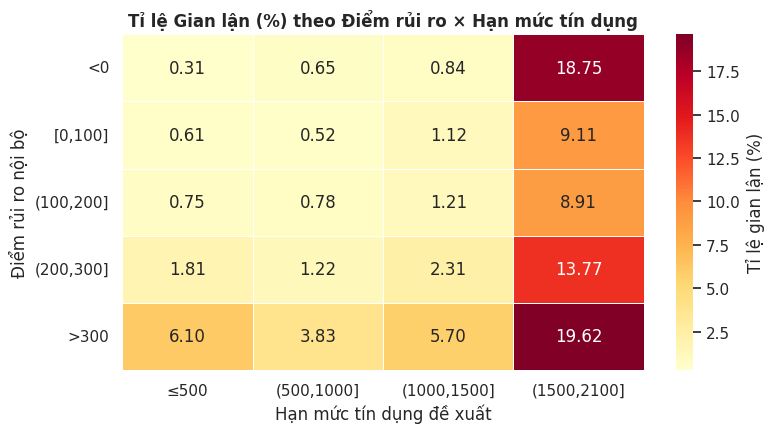
\includegraphics[width=\linewidth]{tabular/c52_f0.png}
  \end{minipage}\hfill
  \begin{minipage}[b]{0.49\linewidth}
    \centering
    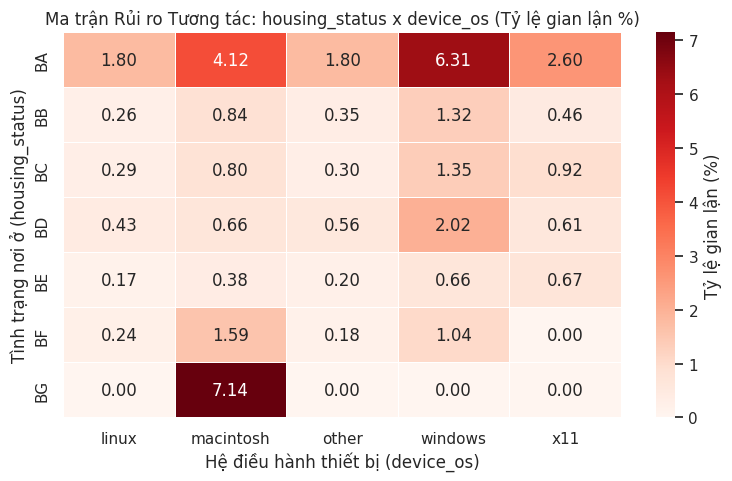
\includegraphics[width=\linewidth]{tabular/c56_f0.png}
  \end{minipage}
  \caption{Bản đồ nhiệt tương tác phi tuyến: điểm rủi ro tín dụng $\times$ hạn mức đề xuất (trái) và tình trạng nhà ở $\times$ hệ điều hành thiết bị (phải).}
  \label{fig:tab_interactions}
\end{figure}

Đánh giá toàn diện 31 thuộc tính còn lại bằng Thông tin tương hỗ (\textit{Mutual Information -- MI}) cho thấy các biến phân loại và cờ hành vi dẫn đầu về khả năng phân tách phi tuyến (\texttt{housing\_status}: 0,0367; \texttt{prev\_address\_months\_count}: 0,0288; \texttt{device\_os}: 0,0258; \texttt{keep\_alive\_session}: 0,0244; \texttt{intended\_balcon\_amount}: 0,0233). Kiểm tra chỉ số ổn định phân phối (\textit{Population Stability Index -- PSI}) giữa nửa đầu (tháng 0--2) và nửa sau (tháng 3--5) của tập Train cho thấy phần lớn biến ổn định ($\text{PSI} < 0,10$), ngoại trừ nhóm vận tốc biến động mạnh theo mùa vụ (\texttt{velocity\_4w}: 4,1643; \texttt{velocity\_24h}: 0,6191; \texttt{velocity\_6h}: 0,2925) và \texttt{credit\_risk\_score} (0,2744).

\subsubsection{Chênh lệch nhân khẩu học và tiền đề đánh giá công bằng}
Khảo sát các thuộc tính nhạy cảm (\Cref{fig:tab_demo}) cho thấy tỷ lệ gian lận tăng đều theo độ tuổi: từ 0,33\% ở nhóm 10 tuổi và 0,45\% ở nhóm 20 tuổi lên 1,12\% ở tuổi 40 và 3,08\% ở tuổi 60 (theo \cite{jesus2022turning}, kẻ gian thường nhắm mạo danh người lớn tuổi do nhóm này có uy tín tín dụng cao hơn). Khi tách theo ngưỡng 50 tuổi, nhóm $\ge 50$ tuổi chỉ chiếm 18,77\% hồ sơ (149.234 đơn) nhưng có tỷ lệ gian lận 2,21\%, gấp \textbf{2,94 lần} nhóm $< 50$ tuổi (0,75\% trên 645.755 đơn). Tương tự, tỷ số chênh lệch (\textit{Disparity Ratio}) giữa nhóm thu nhập cao ($> 0,6$: 1,33\%) và thu nhập thấp ($\le 0,3$: 0,58\%) là 2,28 lần, còn giữa nhóm nghề nghiệp \texttt{CC} và \texttt{CF} là 12,45 lần. Sự khác biệt về tỷ lệ nền (\textit{prevalence}) này báo trước nguy cơ một mô hình dùng ngưỡng phân loại chung sẽ gây tỷ lệ báo động nhầm cao hơn nhiều cho nhóm khách hàng lớn tuổi.

\begin{figure}[H]
  \centering
  \begin{minipage}[b]{0.47\linewidth}
    \centering
    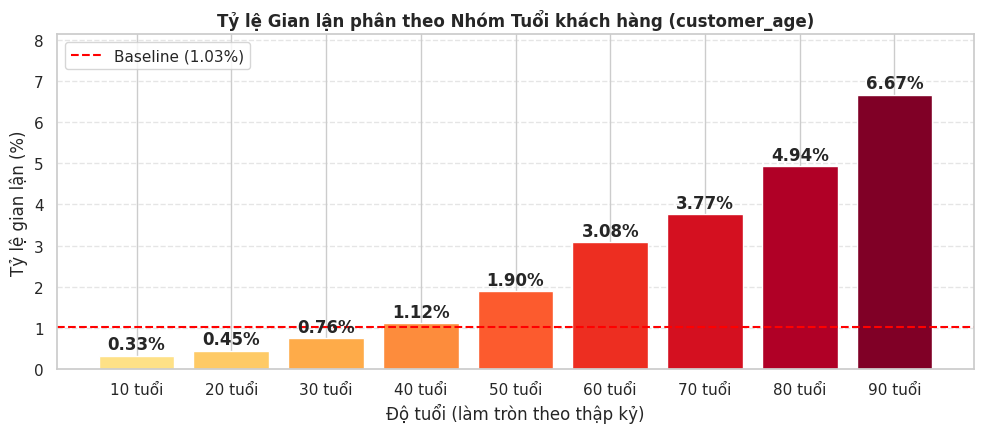
\includegraphics[width=\linewidth]{tabular/c62_f0.png}
  \end{minipage}\hfill
  \begin{minipage}[b]{0.51\linewidth}
    \centering
    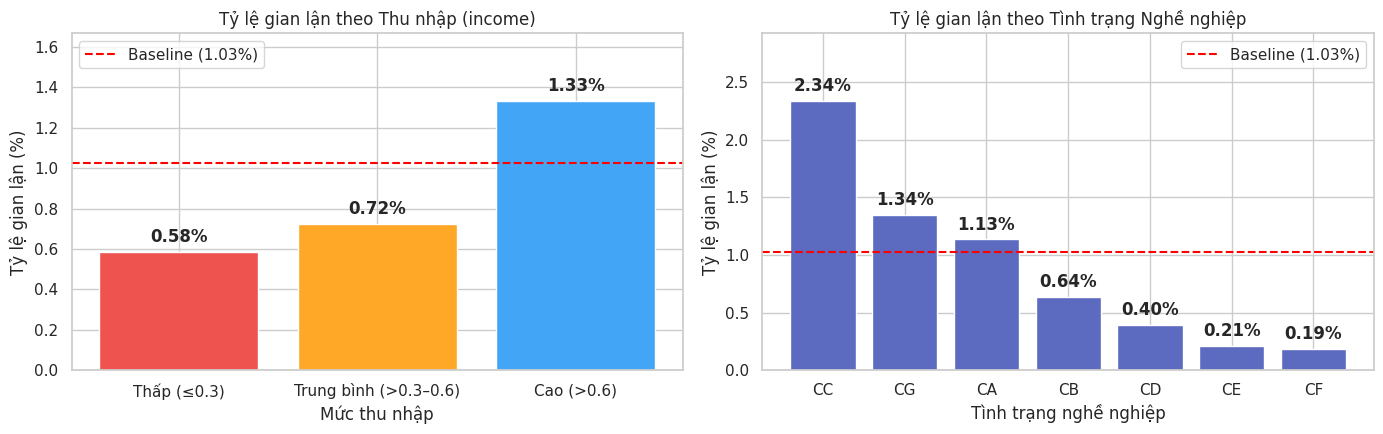
\includegraphics[width=\linewidth]{tabular/c66_f0.png}
  \end{minipage}
  \caption{Tỷ lệ gian lận tăng dần theo độ tuổi (trái) và chênh lệch rủi ro nền theo mức thu nhập, tình trạng nghề nghiệp (phải) trên \texttt{df\_train}.}
  \label{fig:tab_demo}
\end{figure}

\subsection{Tiền xử lý, kỹ thuật đặc trưng và thiết lập mô hình}
Nhằm giúp mô hình cây nắm bắt các quan hệ tỷ lệ và giảm tác động của trôi dạt vận tốc theo mùa vụ, nhóm bổ sung \textbf{6 đặc trưng tỷ lệ} gồm: hai tỷ lệ vận tốc ngắn/dài hạn (\texttt{vel\_6h\_24h}, \texttt{vel\_24h\_4w}), thâm niên cư trú và ngân hàng chuẩn hóa theo tuổi (\texttt{addr\_per\_age}, \texttt{bank\_per\_age}), và hai tỷ lệ hạn mức, tiền nạp so với thu nhập (\texttt{limit\_per\_income}, \texttt{balcon\_per\_income}). Tổng cộng đầu vào gồm \textbf{42 đặc trưng} (36 biến số bao gồm 6 cờ \texttt{\_flag} và 6 tỷ lệ mới, 5 biến phân loại, cùng biến \texttt{month}). Thử nghiệm \textit{ablation} với 3 seed trên biến \texttt{month} cho thấy việc loại bỏ \texttt{month} làm \texttt{TPR@5\%FPR} thay đổi $+0,010$ (CI 95\% $[-0,015; +0,022]$, không có ý nghĩa thống kê); do đó \texttt{month} được giữ lại như lựa chọn nhất quán giữa các bảng thực nghiệm, đi kèm lưu ý biến này không thể ngoại suy vượt ngoài miền tháng 0--5.

Để chọn phương pháp chuẩn hóa cho mô hình tuyến tính, \Cref{fig:tab_scaling} đối chiếu phân phối gốc với \texttt{StandardScaler} và \texttt{RobustScaler} trên \texttt{velocity\_6h} và \texttt{intended\_balcon\_amount}. Nhờ dựa trên trung vị và khoảng tứ phân vị (IQR), \texttt{RobustScaler} giữ nguyên cấu trúc phân phối và hạn chế hiện tượng co cụm dữ liệu bình thường do ảnh hưởng của ngoại lai.

\begin{figure}[H]
  \centering
  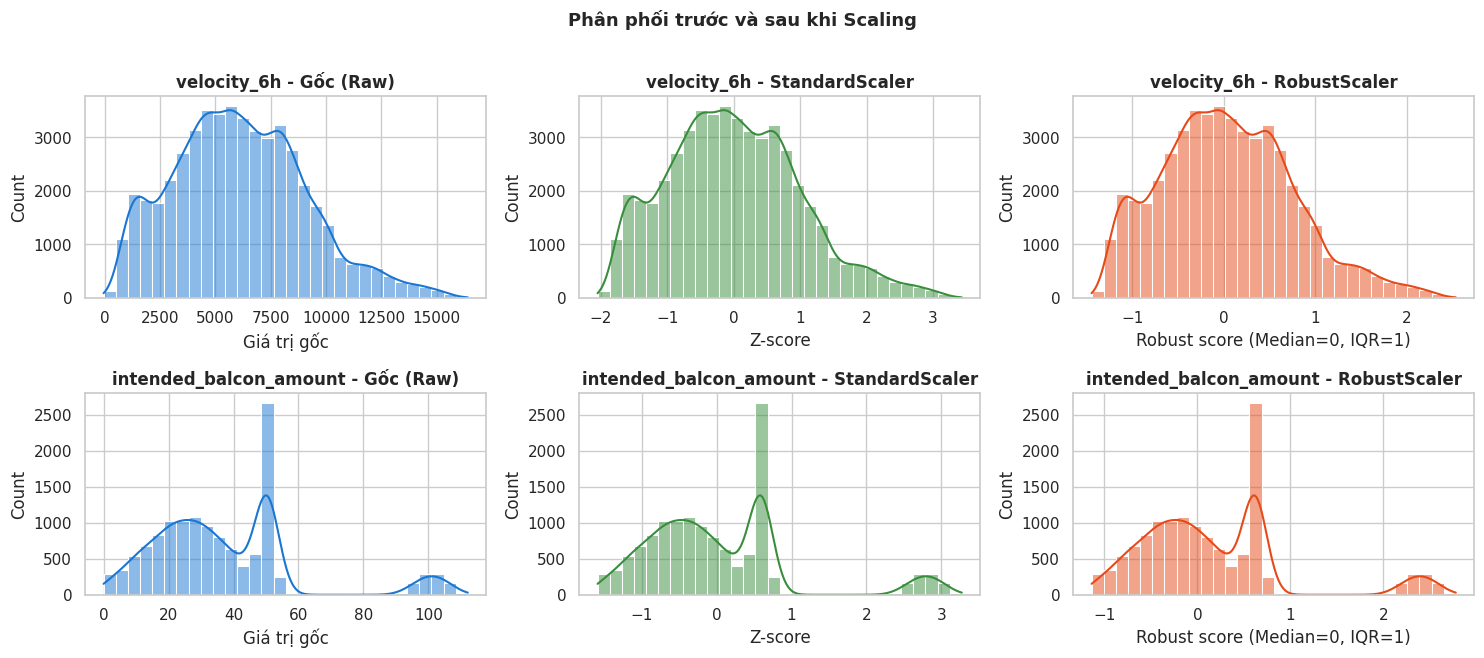
\includegraphics[width=0.90\linewidth]{tabular/c68_f0.png}
  \caption{Phân phối của \texttt{velocity\_6h} và \texttt{intended\_balcon\_amount} trước và sau chuẩn hóa bằng \texttt{StandardScaler} và \texttt{RobustScaler} trên \texttt{df\_train}.}
  \label{fig:tab_scaling}
\end{figure}

Hai họ mô hình được huấn luyện theo quy trình tách biệt hoàn toàn trên \texttt{df\_train}:
\begin{itemize}[leftmargin=*]
  \item \textbf{Logistic Regression (mô hình cơ sở):} sử dụng \texttt{SimpleImputer(median)}, \texttt{RobustScaler} và \texttt{OneHotEncoder} đóng gói trong \texttt{Pipeline}, kèm tham số \texttt{class\_weight='balanced'} để bù mất cân bằng lớp.
  \item \textbf{LightGBM (mô hình chính):} giữ nguyên giá trị \texttt{NaN}, xử lý trực tiếp biến phân loại dạng \texttt{category}, sử dụng siêu tham số tham khảo từ \cite{jesus2022turning} với dừng sớm (\textit{early stopping}) theo Validation AUC và lấy trung bình dự đoán từ 3 seed độc lập (số cây tối ưu lần lượt là 438, 637 và 531 cây) nhằm giảm phương sai ước lượng.
\end{itemize}

Ngưỡng phân loại được chọn duy nhất trên Validation (tháng 6) tại điểm $\text{FPR} \le 5\%$ — thu được ngưỡng \textbf{0,7781} cho Logistic Regression và \textbf{0,0478} cho LightGBM — sau đó khóa cứng để đánh giá một lần trên Test (tháng 7).

\subsection{Kết quả thực nghiệm, giải thích mô hình và kiểm chứng giả thuyết}

\subsubsection{Hiệu năng phân loại, đối chiếu tài liệu gốc và kiểm định Bootstrap}
\Cref{tab:tab_results} tổng hợp kết quả của hai mô hình trên Validation và Test, đặt cạnh mốc tham chiếu của bài báo gốc NeurIPS 2022 \cite{jesus2022turning}. Trên tập Test (96.843 hồ sơ, 1.428 ca gian lận), LightGBM đạt \texttt{TPR@FPR5\%} xếp hạng bằng \textbf{0,5798}, tái lập sát và nhỉnh hơn mốc 0,5600 công bố trong bài báo gốc. Khi khóa ngưỡng từ tháng 6 sang tháng 7 (\texttt{TPR@ngưỡng}), LightGBM phát hiện được 793 ca gian lận (55,53\%, giảm 19,0\% số ca bỏ lọt so với 644 ca của Logistic Regression) với FPR thực tế ở mức 4,22\%, vẫn nằm trong ngân sách 5\%. Khoảng cách giữa \texttt{TPR@FPR5\%} (0,580) và \texttt{TPR@ngưỡng} (0,555) phản ánh hiện tượng ngưỡng cố định trở nên chặt hơn khi tỷ lệ gian lận tháng 7 tăng cao, gợi ý cần hiệu chỉnh lại ngưỡng định kỳ theo phân vị lưu lượng cảnh báo khi vận hành.

\begin{table}[H]
  \centering
  \caption{Hiệu năng Logistic Regression và LightGBM trên Validation (tháng 6), Test (tháng 7) và đối chiếu với mốc bài báo gốc \cite{jesus2022turning}.}
  \label{tab:tab_results}
  \resizebox{\linewidth}{!}{%
  \begin{tabular}{l l c c c c c c}
    \toprule
    \textbf{Tập / Nguồn} & \textbf{Mô hình} & \textbf{TPR@FPR5\%} & \textbf{TPR@ngưỡng} & \textbf{FPR} & \textbf{Precision} & \textbf{ROC-AUC} & \textbf{PR-AUC} \\
    \midrule
    Val (Tháng 6) & Logistic Regression & 0,5069 & 0,5069 & 0,0495 & 0,1221 & 0,8829 & 0,1565 \\
    Val (Tháng 6) & LightGBM & 0,5310 & 0,5310 & 0,0496 & 0,1270 & 0,8948 & 0,1822 \\
    \midrule
    Test (Tháng 7) & Logistic Regression & 0,5301 & 0,4510 & 0,0348 & 0,1624 & 0,8868 & 0,1849 \\
    Test (Tháng 7) & LightGBM & \textbf{0,5798} & \textbf{0,5553} & 0,0422 & \textbf{0,1647} & \textbf{0,8986} & \textbf{0,2173} \\
    \midrule
    Paper \cite{jesus2022turning} & Logistic Regression & $\sim 0,5100$ & -- & 0,0500 & -- & -- & -- \\
    Paper \cite{jesus2022turning} & LightGBM & 0,5600 & -- & 0,0500 & -- & -- & -- \\
    \bottomrule
  \end{tabular}%
  }
\end{table}

Do tập Test chỉ chứa 1.428 ca gian lận, sai số lấy mẫu có thể lên tới $\pm 0,025$ điểm TPR. Kết quả lấy mẫu cặp \textit{Bootstrap} phân tầng 1.000 lần (\Cref{tab:tab_bootstrap}) cho thấy khoảng tin cậy 95\% của chênh lệch giữa LightGBM và Logistic Regression hoàn toàn nằm trên 0 ở cả ba chỉ số (\texttt{TPR@FPR5\%}: $+0,050$; \texttt{TPR@ngưỡng}: $+0,104$; \texttt{ROC-AUC}: $+0,012$), xác nhận lợi thế của mô hình cây có ý nghĩa thống kê. Đường cong ROC, Precision-Recall và ma trận nhầm lẫn tương ứng được thể hiện ở \Cref{fig:tab_roc_cm}.

\begin{table}[H]
  \centering
  \caption{Khoảng tin cậy Bootstrap 95\% (1.000 mẫu phân tầng) trên tập Test tháng 7.}
  \label{tab:tab_bootstrap}
  \resizebox{\linewidth}{!}{%
  \begin{tabular}{l c c c c}
    \toprule
    \textbf{Chỉ số} & \textbf{Logistic Regression} & \textbf{LightGBM} & \textbf{Chênh lệch (LGBM $-$ LR)} & \textbf{Ý nghĩa (95\%)} \\
    \midrule
    TPR@FPR5\% (xếp hạng) & 0,530 $[0,505;\; 0,557]$ & 0,580 $[0,554;\; 0,605]$ & $+0,050$ $[+0,031;\; +0,068]$ & Có \\
    TPR@ngưỡng (triển khai) & 0,451 $[0,425;\; 0,478]$ & 0,555 $[0,529;\; 0,582]$ & $+0,104$ $[+0,085;\; +0,123]$ & Có \\
    ROC-AUC & 0,887 $[0,878;\; 0,895]$ & 0,899 $[0,891;\; 0,906]$ & $+0,012$ $[+0,009;\; +0,015]$ & Có \\
    \bottomrule
  \end{tabular}%
  }
\end{table}

\begin{figure}[H]
  \centering
  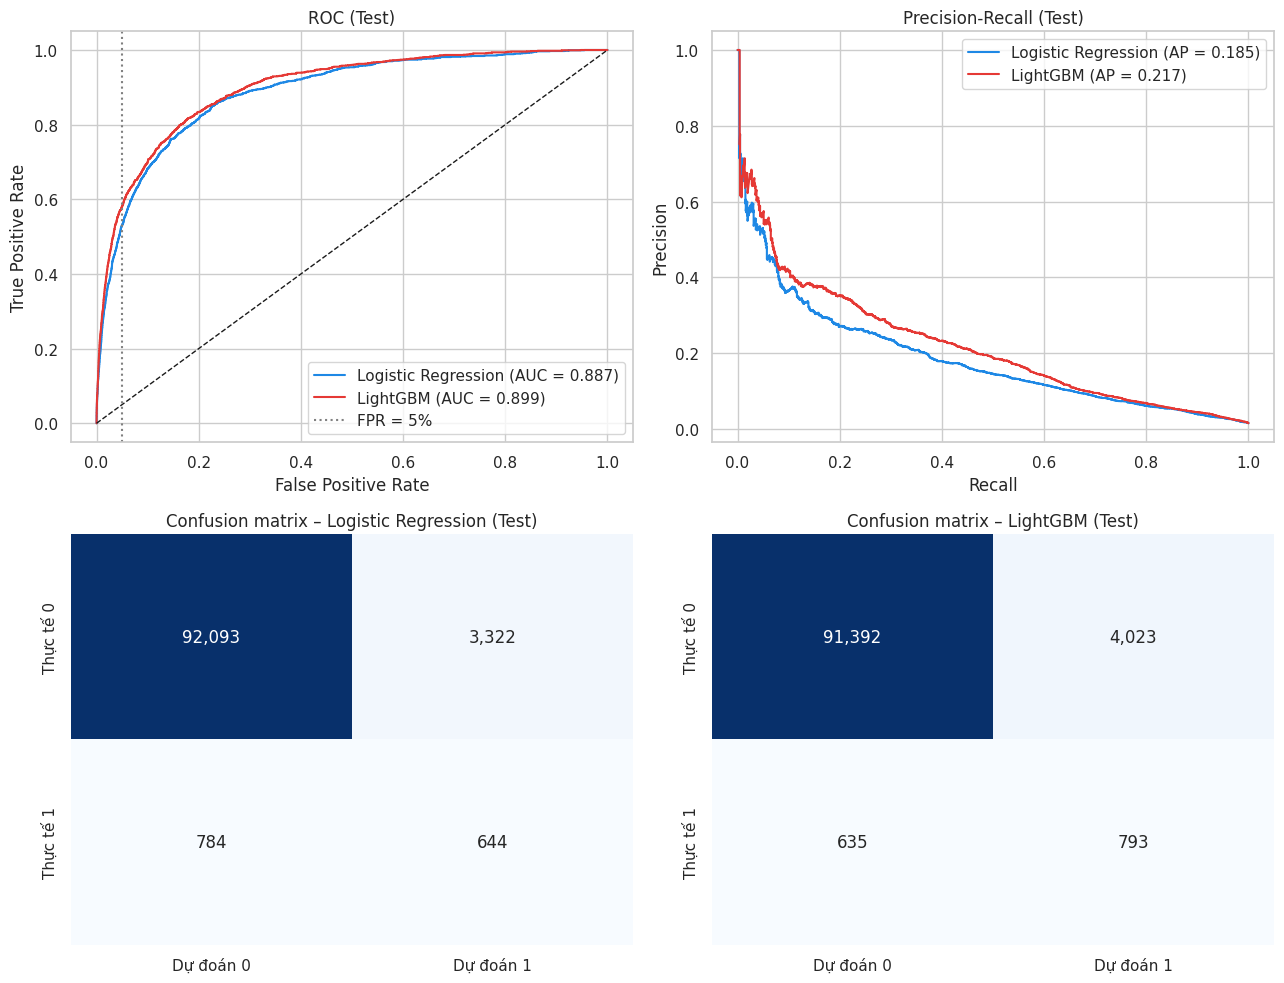
\includegraphics[width=0.90\linewidth]{tabular/c84_f0.png}
  \caption{Đường cong ROC, Precision-Recall và ma trận nhầm lẫn của Logistic Regression và LightGBM trên tập Test (tháng 7).}
  \label{fig:tab_roc_cm}
\end{figure}

\subsubsection{Đóng góp đặc trưng và độ hiệu chỉnh xác suất}
Phân tích mức độ đóng góp đặc trưng theo chỉ số \textit{Gain} trung bình qua 3 seed của LightGBM (\Cref{fig:tab_feat_imp}) cho thấy nhiều đặc trưng thiết kế trực tiếp từ giả thuyết EDA — như \texttt{limit\_per\_income}, \texttt{addr\_per\_age}, \texttt{bank\_per\_age} và cờ \texttt{prev\_address\_months\_count\_flag} — đều nằm trong nhóm 15 biến quan trọng nhất. Về độ hiệu chỉnh xác suất (\textit{Calibration}), LightGBM không điều chỉnh trọng số lớp nên bảo toàn xác suất tiên nghiệm, đạt \textit{Brier Score} trên Test bằng \textbf{0,01283} (có thể dùng trực tiếp để ước lượng tổn thất kỳ vọng); trái lại, Logistic Regression với \texttt{class\_weight='balanced'} làm xác suất đầu ra bị khuếch đại (\textit{Brier Score} = 0,09944), chỉ phù hợp cho mục đích xếp hạng.

\begin{figure}[H]
  \centering
  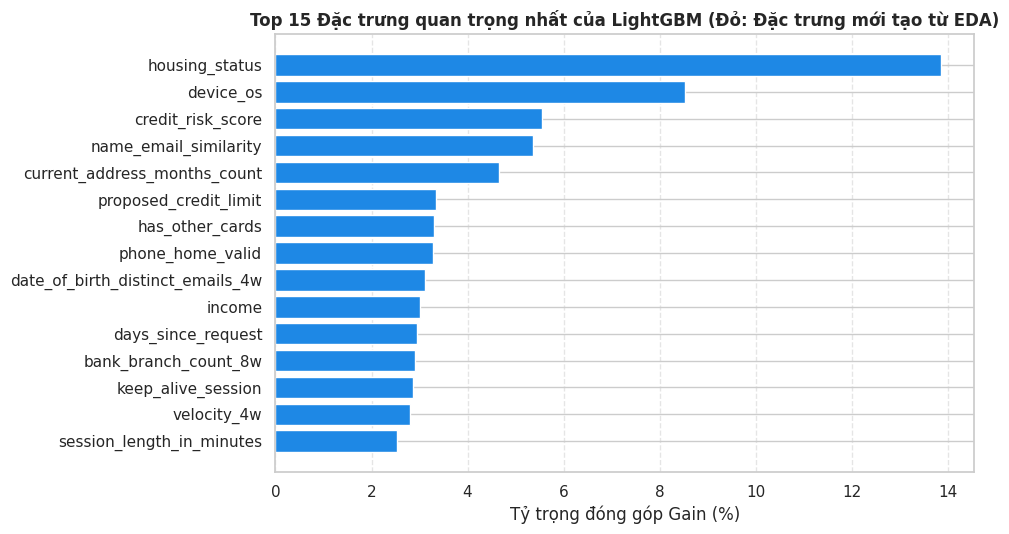
\includegraphics[width=0.84\linewidth]{tabular/c87_f0.png}
  \caption{Top 15 đặc trưng có tỷ trọng đóng góp \textit{Gain} lớn nhất trong LightGBM (màu đỏ đánh dấu các đặc trưng mới tạo từ phân tích EDA).}
  \label{fig:tab_feat_imp}
\end{figure}

\subsubsection{Đánh giá công bằng theo nhóm tuổi và đánh đổi vận hành}
Khi áp dụng ngưỡng chung 0,0478 của LightGBM trên tập Test (\Cref{fig:tab_fairness_policy}), tỷ lệ báo động nhầm của nhóm $\ge 50$ tuổi (12.667 hồ sơ) lên tới \textbf{10,12\%}, gấp ba lần nhóm $< 50$ tuổi (3,35\% trên 84.176 hồ sơ), kéo chỉ số $\text{FPR ratio} = \text{FPR}(<50)/\text{FPR}(\ge 50)$ xuống còn \textbf{0,331}. Việc áp ngưỡng riêng cho từng nhóm trên Validation đưa tỷ lệ báo động nhầm về trạng thái cân bằng (4,63\% so với 4,56\%, $\text{FPR ratio} = \mathbf{1,014}$), nhưng kéo theo sự sụt giảm rõ rệt về khả năng phát hiện gian lận ở nhóm $\ge 50$ tuổi (TPR giảm từ 71,29\% xuống 52,63\%, TPR toàn cục giảm từ 55,53\% xuống 54,20\%).

Hai thực nghiệm phụ được thực hiện để làm rõ cơ chế thiên lệch. Thứ nhất, khi loại bỏ hoàn toàn \texttt{customer\_age} và hai biến tỷ lệ chứa tuổi (\textit{Fairness through Unawareness}), FPR nhóm $\ge 50$ tuổi vẫn giữ ở mức 8,68\% so với 3,68\% của nhóm trẻ ($\text{FPR ratio} = 0,425$). Một mô hình phụ huấn luyện trên các biến còn lại vẫn dự đoán được nhóm tuổi $\ge 50$ với \textbf{AUC = 0,835}, chứng tỏ thông tin tuổi bị rò rỉ mạnh qua các biến gián tiếp (\textit{proxy leakage}), bên cạnh chênh lệch tỷ lệ gian lận nền vốn có. Thứ hai, khảo sát điểm đánh đổi trung gian với mục tiêu FPR 6,5\% trên Validation cho nhóm $\ge 50$ tuổi đạt FPR thực tế 6,01\% và giữ được TPR 59,33\% trên Test. Trong thực tiễn, thay vì tự động từ chối hồ sơ bằng ngưỡng phân biệt theo tuổi (có thể vướng quy định pháp lý), hướng tiếp cận phù hợp hơn là chuyển các hồ sơ bị cảnh báo sang bước xác thực bổ sung hoặc duyệt thủ công kết hợp giám sát FPR/TPR định kỳ theo nhóm nhân khẩu học.

\begin{figure}[H]
  \centering
  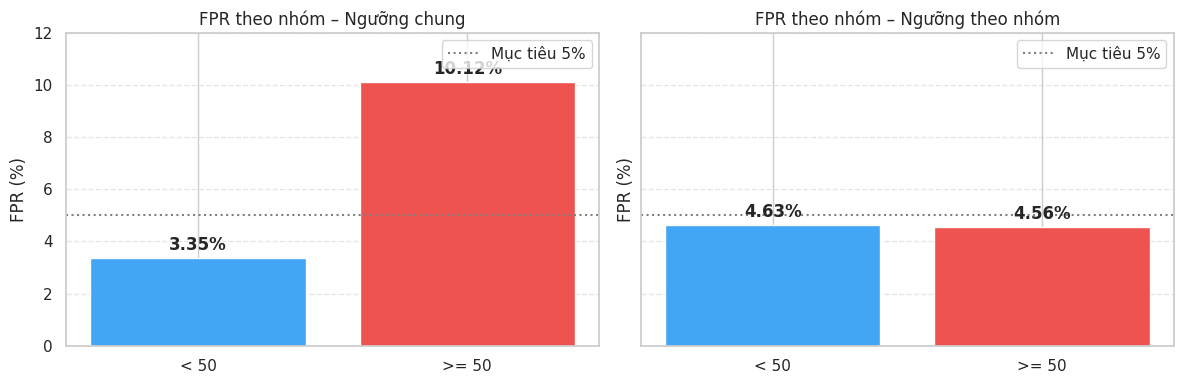
\includegraphics[width=0.86\linewidth]{tabular/c90_f0.png}
  \caption{So sánh tỷ lệ báo động nhầm (FPR) giữa hai nhóm tuổi dưới chính sách ngưỡng chung ($\text{FPR ratio} = 0,331$) và ngưỡng riêng theo nhóm ($\text{FPR ratio} = 1,014$).}
  \label{fig:tab_fairness_policy}
\end{figure}

\subsubsection{Kiểm chứng thực nghiệm giả thuyết EDA và phương pháp chia tập}
Hai thực nghiệm đối chứng cuối cùng trên cả Logistic Regression và LightGBM (\Cref{fig:tab_ablations}) xác nhận hai quyết định thiết kế nền tảng của bài toán:
\begin{enumerate}[leftmargin=*]
  \item \textbf{Tác động của 6 cột khuyết và 6 cờ \texttt{\_flag}:} Khi loại bỏ hoàn toàn nhóm đặc trưng này (còn 27 biến), \texttt{TPR@FPR5\%} giảm từ 0,5301 xuống 0,5035 ở Logistic Regression và từ 0,5798 xuống 0,5448 ở LightGBM (\texttt{ROC-AUC} giảm từ 0,8986 xuống 0,8837). Đáng chú ý, nếu chỉ bỏ 6 cờ \texttt{\_flag} và giữ 6 cột gốc, Logistic Regression sụt giảm ngay (0,5301 $\rightarrow$ 0,5056) vì phép điền trung vị xóa mất dấu hiệu MNAR, còn LightGBM gần như giữ nguyên (0,5749) nhờ cơ chế rẽ nhánh mặc định cho \texttt{NaN}. Kết hợp giữ \texttt{NaN} và 6 cờ \texttt{\_flag} vì thế mang lại lợi ích nhất quán cho cả hai họ mô hình.
  \item \textbf{Temporal Split so với Stratified Random Split:} Chia ngẫu nhiên 80/10/10 trộn lẫn cả 8 tháng tạo ra độ lạc quan giả tạo khi đánh giá (ngay cả khi lọc riêng lát cắt tháng 7 trong tập Test ngẫu nhiên, \texttt{TPR@ngưỡng} của Logistic Regression bị đẩy từ 0,4510 lên 0,4915 và của LightGBM lên 0,5763). Quan trọng hơn, ngưỡng chọn từ tập Validation trộn lẫn không phản ánh sự dịch chuyển của tháng 7, khiến FPR của LightGBM trên lát cắt tháng 7 tăng vọt lên \textbf{6,34\%}, phá vỡ ngân sách $\le 5\%$.
\end{enumerate}

\begin{figure}[H]
  \centering
  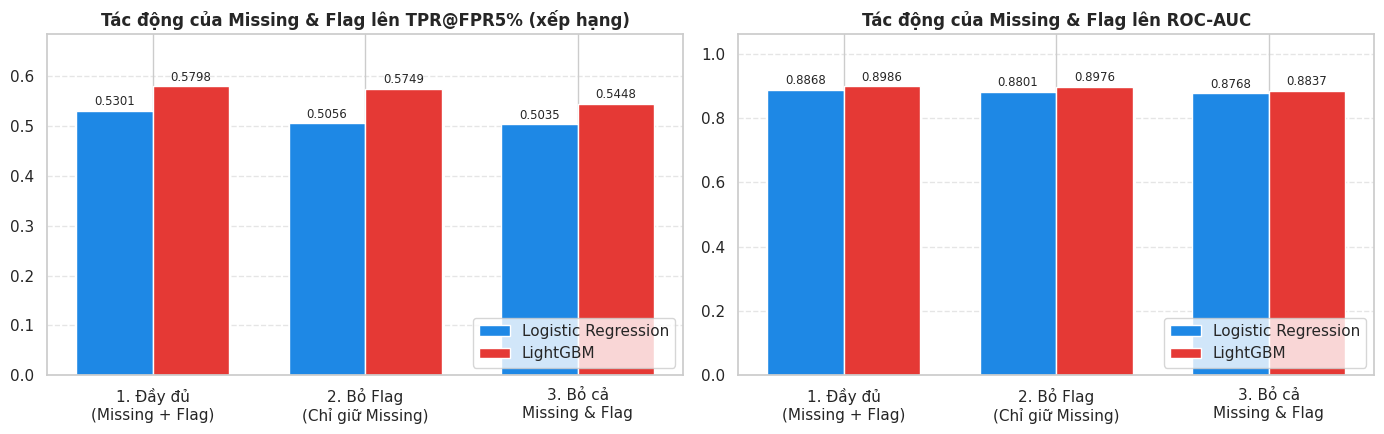
\includegraphics[width=0.90\linewidth]{tabular/c96_f0.png}\\[4pt]
  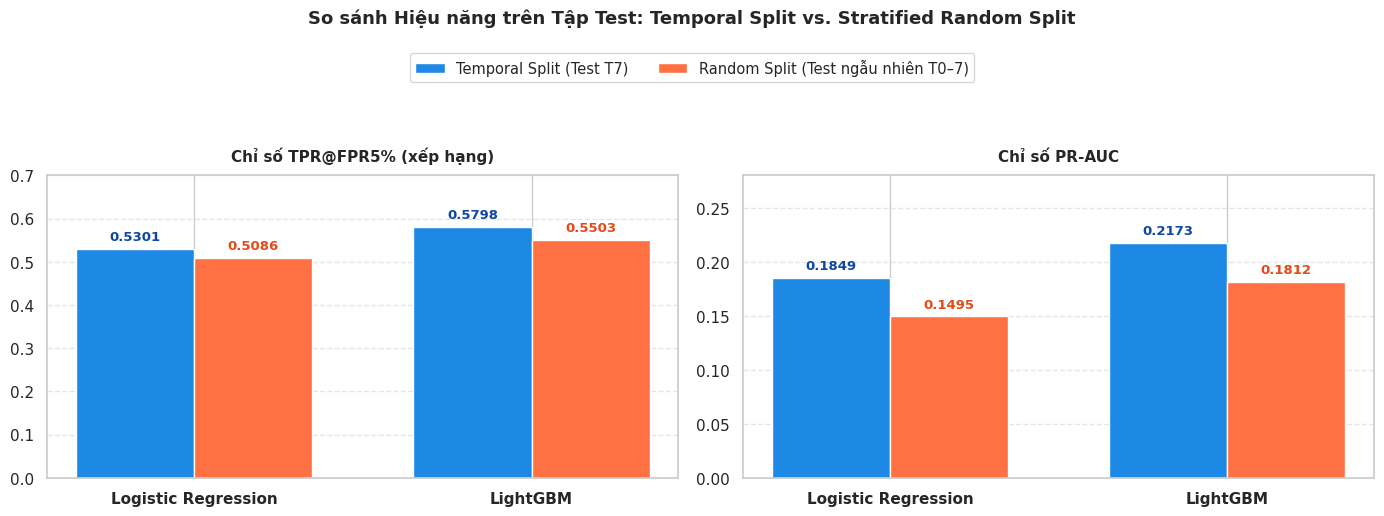
\includegraphics[width=0.90\linewidth]{tabular/c99_f0.png}
  \caption{Hai thực nghiệm kiểm chứng trên tập Test: tác động khi loại bỏ cột khuyết và cờ \texttt{\_flag} (trên) và so sánh \textit{Temporal Split} với \textit{Stratified Random Split} (dưới).}
  \label{fig:tab_ablations}
\end{figure}

\section{Dữ liệu văn bản: Phân loại tin tức kinh tế -- tài chính tiếng Việt}
\label{sec:text}

\subsection{Thu thập dữ liệu và Chuẩn hóa tiếng Việt}
Thay vì dùng tập có sẵn, nhóm tự xây dựng bộ thu thập (\textit{crawler}) từ trang báo \textbf{VnEconomy} (giai đoạn 05/11/2025 -- 21/11/2026), thu được tập dữ liệu cân bằng gồm \textbf{5.000 bài viết} chia đều cho \textbf{5 chuyên mục} (1.000 bài/lớp): \textit{Bất động sản}, \textit{Chứng khoán}, \textit{Thế giới}, \textit{Thị trường}, và \textit{Tài chính}. Kiểm tra toàn vẹn cho thấy 0 giá trị thiếu, 0 trùng lặp ID/URL/nội dung.

Ở bước chuẩn hóa tiếng Việt:
\begin{itemize}[leftmargin=*]
  \item Chuyển 193 bài chưa chuẩn mã Unicode sang dạng dựng sẵn \textbf{NFC}.
  \item Thống nhất quy tắc bỏ dấu kiểu cũ (94.955 từ) sang kiểu mới (tổng 119.799 từ chuẩn hóa, ví dụ: \textit{hòa bình, thủy sản, Ủy ban}) để tránh phân mảnh từ vựng.
  \item Tách từ tiếng Việt bằng thư viện \texttt{underthesea}, rút gọn từ trung bình 1.075 âm tiết/bài xuống 737 token/bài (tổng 3.684.703 token, 55.653 từ vựng duy nhất; lọc từ xuất hiện $\ge 5$ bài còn 9.497 từ nhưng vẫn phủ 97,9\% tổng token).
\end{itemize}

\subsection{Khám phá dữ liệu (EDA) và Phát hiện rò rỉ thông tin}
Phân tích EDA chỉ ra ba đặc điểm quan trọng ảnh hưởng trực tiếp đến thiết kế mô hình:
\begin{enumerate}[leftmargin=*]
  \item \textbf{Độ dài văn bản (\Cref{fig:text_length}):} Trung vị độ dài các lớp dao động từ 894,5 âm tiết (\textit{Chứng khoán}) đến 1.128,0 âm tiết (\textit{Thị trường}). Kiểm định Kruskal-Wallis ($H = 105,7, p = 6{,}0\times 10^{-22}, \eta^2 = 0{,}020$) cho thấy sự khác biệt độ dài có ý nghĩa thống kê nhưng kích thước hiệu ứng nhỏ, không thể dùng độ dài làm đặc trưng phân loại chính.
  \item \textbf{Bài gần trùng và chuỗi tin định kỳ (\Cref{fig:text_dup}):} Dùng độ tương đồng Cosine trên TF-IDF với ngưỡng $0,90$, nhóm phát hiện \textbf{18 nhóm gần trùng} gồm \textbf{248 bài (5,0\%)}, tập trung mạnh ở \textit{Tài chính} (141 bài) và \textit{Chứng khoán} (86 bài), trong đó nhóm lớn nhất có tới 125 bản tin định kỳ. Nếu chia tập ngẫu nhiên, các bài gần trùng sẽ lọt vào cả Train và Test, gây ảo giác độ chính xác.
  \item \textbf{Từ khóa đặc trưng và rò rỉ tên tác giả (\Cref{fig:text_keywords,fig:text_author}):} Phân tích \textit{Log-odds Z-score} cho thấy các từ khóa phân tách rõ rệt theo chuyên mục (khi loại bỏ chuỗi lặp, 9--10/10 từ khóa top đầu ở 4 lớp vẫn giữ nguyên, riêng \textit{Tài chính} giữ 6/10). Đáng chú ý, chỉ dựa vào tên tác giả (\texttt{author\_clean}, 222 tác giả, 10 tác giả đầu viết 46,5\% số bài) đã đoán đúng tới \textbf{92,3\%} chuyên mục (so với 20\% ngẫu nhiên), dù tên tác giả xuất hiện trong nội dung chỉ ở 7 bài.
\end{enumerate}

\begin{figure}[H]
  \centering
  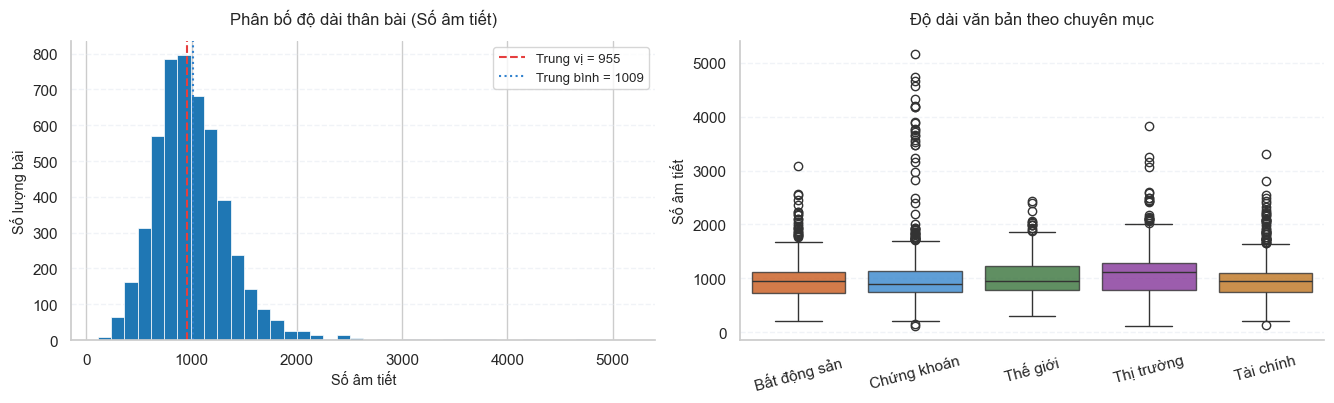
\includegraphics[width=0.86\linewidth]{text/c11_f0.png}
  \caption{Phân phối độ dài bài viết (âm tiết) theo 5 chuyên mục VnEconomy: các chuyên mục có phân phối giao thoa mạnh ($\eta^2 = 0,020$), khẳng định cần dựa vào ngữ nghĩa từ vựng thay vì thống kê độ dài.}
  \label{fig:text_length}
\end{figure}

\begin{figure}[H]
  \centering
  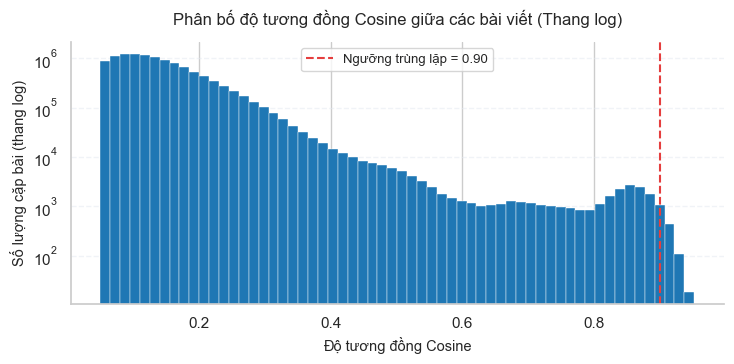
\includegraphics[width=0.86\linewidth]{text/c14_f0.png}
  \caption{Phân tích các cặp bài viết gần trùng (Cosine $\ge 0,90$): phát hiện 18 nhóm (248 bài, 5,0\% tập dữ liệu), là căn cứ để thiết kế phân chia nhóm chống rò rỉ.}
  \label{fig:text_dup}
\end{figure}

\begin{figure}[H]
  \centering
  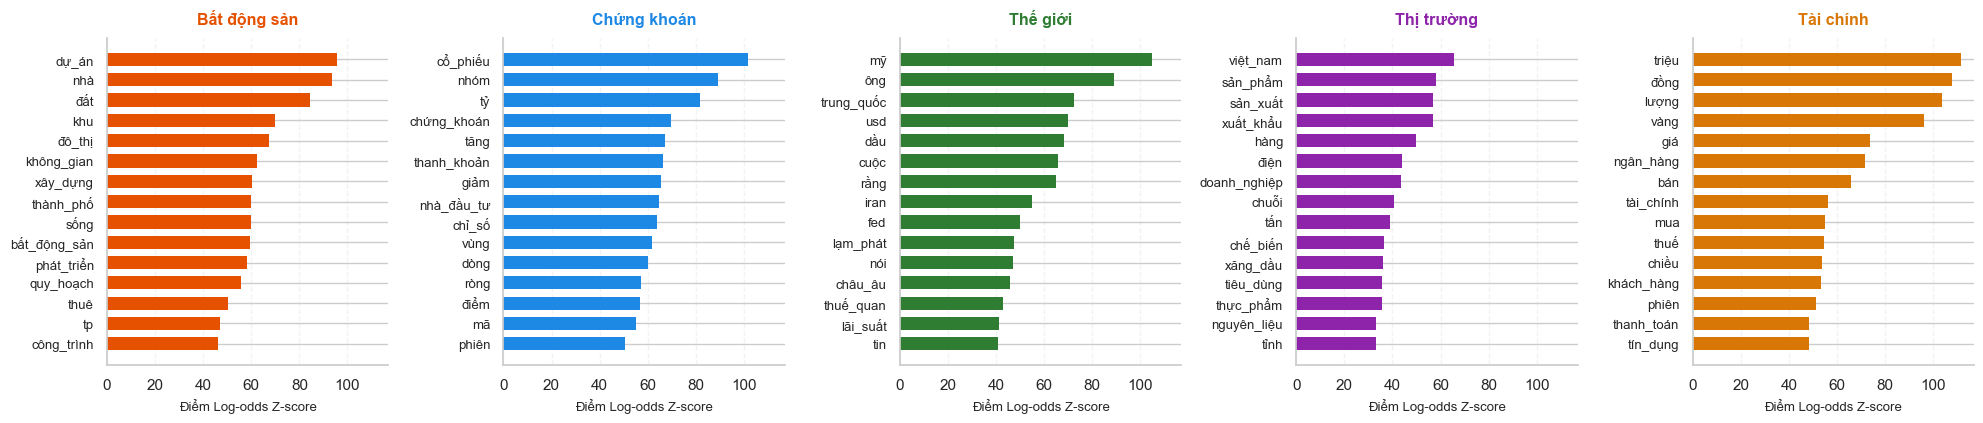
\includegraphics[width=0.88\linewidth]{text/c25_f0.png}
  \caption{Top từ khóa đặc trưng từng chuyên mục theo \textit{Log-odds Z-score}: phản ánh đúng ngữ nghĩa chuyên ngành (ví dụ mã chứng khoán, bất động sản, tỷ giá, địa chính trị).}
  \label{fig:text_keywords}
\end{figure}

\subsection{Thiết kế Pipeline chống rò rỉ và Huấn luyện mô hình}
Để ngăn rò rỉ các bài viết gần trùng, dữ liệu được chia bằng \textbf{StratifiedGroupKFold} theo mã nhóm gần trùng (\texttt{dup\_group}): \textbf{Train/Val} gồm 3.933 bài và \textbf{Test} độc lập gồm 1.067 bài (0 nhóm trùng giữa Train/Val và Test).

Nhóm sử dụng biểu diễn TF-IDF kết hợp tối ưu siêu tham số qua \texttt{GridSearchCV} trên 3 mô hình: \textbf{LinearSVC}, \textbf{Logistic Regression}, và \textbf{Multinomial Naive Bayes}.

\subsection{Kết quả thực nghiệm, Kiểm chứng độ bền và Phân tích lỗi}

\Cref{tab:text_results} và \Cref{fig:text_compare} tổng hợp kết quả đánh giá trên CV và tập Test độc lập (1.067 bài). \textbf{LinearSVC} ($C=100$, n-gram $(1,2)$, bỏ stopword) đạt hiệu năng cao nhất với Test Macro-F1 = \textbf{0,9668} (CI 95\%: $[0,956; 0,977]$), kế đến là Logistic Regression ($0,9603$) và MultinomialNB ($0,9207$). Kiểm định McNemar giữa LinearSVC (1.031/1.067 bài đúng) và Logistic Regression (1.024/1.067 bài đúng) cho $p = 0,118$ (hiệu Macro-F1 $= +0,0066$), cho thấy hai mô hình tuyến tính này tương đương thống kê ở mức $\alpha = 0,05$.

\begin{table}[H]
  \centering
  \caption{Đối chiếu hiệu năng 3 mô hình phân loại văn bản trên Cross-Validation và tập Test độc lập (1.067 bài).}
  \label{tab:text_results}
  \resizebox{\linewidth}{!}{%
  \begin{tabular}{l c c c c}
    \toprule
    \textbf{Mô hình} & \textbf{CV Macro-F1} & \textbf{Test Accuracy} & \textbf{Test Macro-F1} & \textbf{CI 95\% (Test Macro-F1)} \\
    \midrule
    MultinomialNB & $0,9205 \pm 0,0037$ & 0,9203 & 0,9207 & $[0,904;\; 0,936]$ \\
    Logistic Regression & $0,9523 \pm 0,0046$ & 0,9597 & 0,9603 & $[0,949;\; 0,971]$ \\
    LinearSVC & $\mathbf{0,9582 \pm 0,0033}$ & \textbf{0,9663} & \textbf{0,9668} & $\mathbf{[0,956;\; 0,977]}$ \\
    \bottomrule
  \end{tabular}%
  }
\end{table}

\begin{figure}[H]
  \centering
  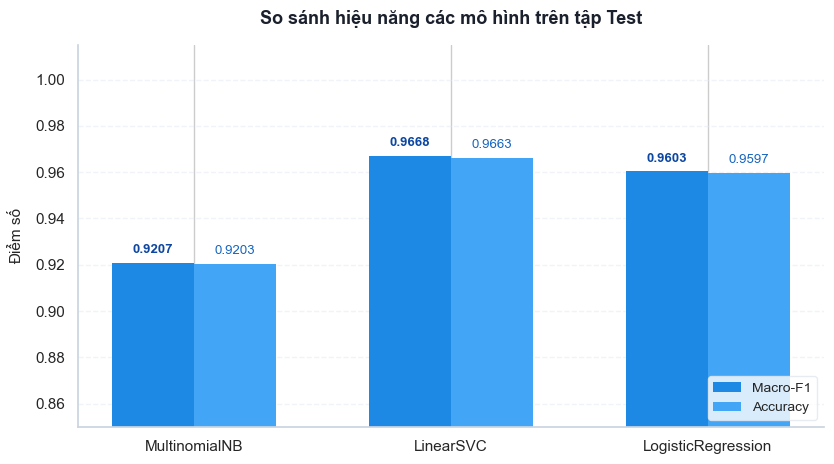
\includegraphics[width=0.86\linewidth]{text/c46_f0.png}
  \caption{So sánh Macro-F1 kèm khoảng tin cậy 95\% trên tập Test (1.067 bài): LinearSVC (0,9668) và Logistic Regression (0,9603) vượt trội rõ rệt so với MultinomialNB (0,9207).}
  \label{fig:text_compare}
\end{figure}

\begin{figure}[H]
  \centering
  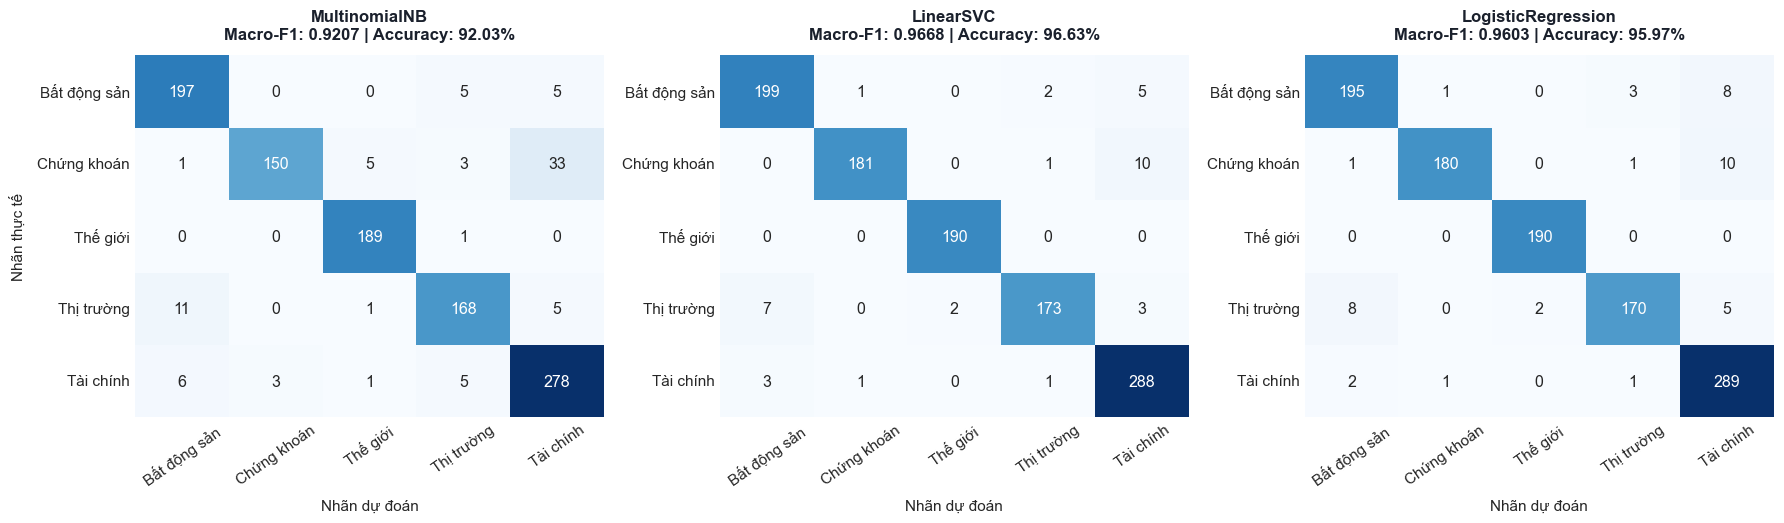
\includegraphics[width=0.82\linewidth]{text/c47_f0.png}
  \caption{Ma trận nhầm lẫn của LinearSVC trên tập Test: lớp \textit{Thế giới} đạt F1 = 0,995; tổng số ca dự đoán sai là 36/1.067 bài, chủ yếu giữa các chuyên mục kinh tế giao thoa như \textit{Tài chính}, \textit{Thị trường} và \textit{Chứng khoán}.}
  \label{fig:text_cm}
\end{figure}

\paragraph{Kiểm chứng độ bền (\textit{Robustness}) và Phân tích lỗi:}
\begin{itemize}[leftmargin=*]
  \item \textbf{Khử trùng hoàn toàn trên Test:} Khi loại bỏ các bài thuộc nhóm gần trùng trên tập Test (còn 939 bài), Macro-F1 của LinearSVC chỉ giảm nhẹ từ $0,9668$ xuống \textbf{0,9611} (Accuracy $= 0,9617$), chứng minh mô hình không học vẹt bản tin lặp.
  \item \textbf{Bóc tách đặc trưng số (\texttt{text\_seg} vs \texttt{text\_num}):} Thay thế số và tỷ lệ phần trăm bằng token đại diện (\texttt{\_so\_}, \texttt{\_pct\_}) giúp CV Macro-F1 tăng nhẹ từ $0,9582 \pm 0,0033$ lên $0,9592 \pm 0,0026$ (giảm phương sai giữa các fold).
  \item \textbf{Kiểm chứng rò rỉ văn phong tác giả (\Cref{fig:text_author}):} Khi chia \texttt{StratifiedGroupKFold} theo \texttt{author\_clean} (đánh giá trên bài của các tác giả chưa từng xuất hiện trong Train), CV Macro-F1 giảm từ $0,9582 \pm 0,0033$ xuống \textbf{0,8519 $\pm$ 0,1030}. Điều này chứng minh một phần hiệu năng cao của mô hình đến từ đặc trưng văn phong riêng của phóng viên chuyên mục.
  \item \textbf{Phân tích 36 ca lỗi trên Test (\Cref{fig:text_cm}):} Có 23 ca nằm ở vùng biên mờ (hiệu điểm top-1 và top-2 $< 0,5$) do giao thoa chủ đề thực sự (ví dụ tin ngân hàng -- chứng khoán -- bất động sản), và 13 ca mô hình tự tin cao ($\ge 0,5$) nhưng gán nhầm nhãn chuyên mục của tòa soạn.
\end{itemize}

\begin{figure}[H]
  \centering
  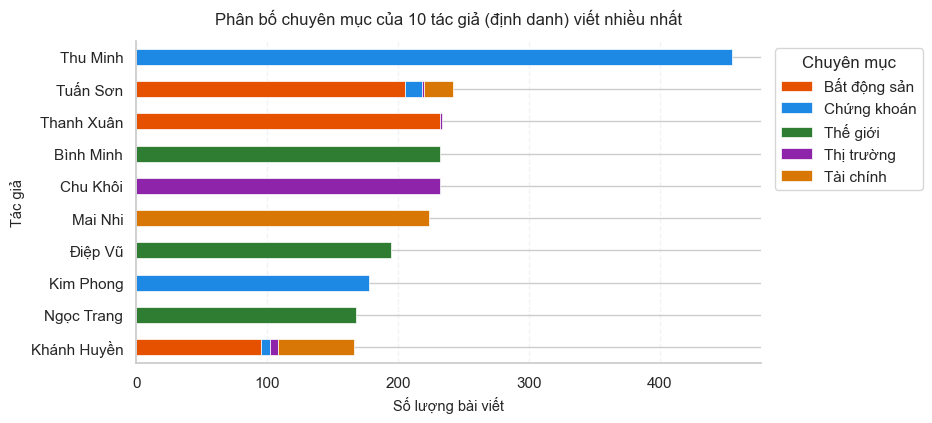
\includegraphics[width=0.84\linewidth]{text/c36_f0.png}
  \caption{Phân bố bài viết theo tác giả: 10 tác giả viết nhiều nhất chiếm 46,5\% tổng số bài, giải thích vì sao chỉ dùng tên tác giả đã đoán đúng 92,3\% chuyên mục và làm CV giảm xuống 0,8519 khi chia tách theo tác giả.}
  \label{fig:text_author}
\end{figure}

\section{Dữ liệu ảnh: Phân loại cảnh quan tự nhiên (Intel Image)}
\label{sec:image}

\subsection{Dữ liệu và Khám phá đặc trưng thị giác (EDA)}
Bài toán sử dụng bộ \textit{Intel Image Classification} \cite{bansal2019intel} gồm \textbf{17.034 ảnh RGB} thuộc \textbf{6 lớp} (\textit{buildings, forest, glacier, mountain, sea, street}), chia sẵn thành 14.034 ảnh Train và 3.000 ảnh Test độc lập. Kiểm tra toàn vẹn cho thấy 0 tệp lỗi, 100\% ảnh ở chế độ 3 kênh màu RGB, đa số kích thước $150\times 150$ px (đạt chuẩn $\ge 128$ px của Assignment v4; một số ít ảnh có chiều cao nhỏ hơn được chuẩn hóa bằng resize/padding).

\begin{figure}[H]
  \centering
  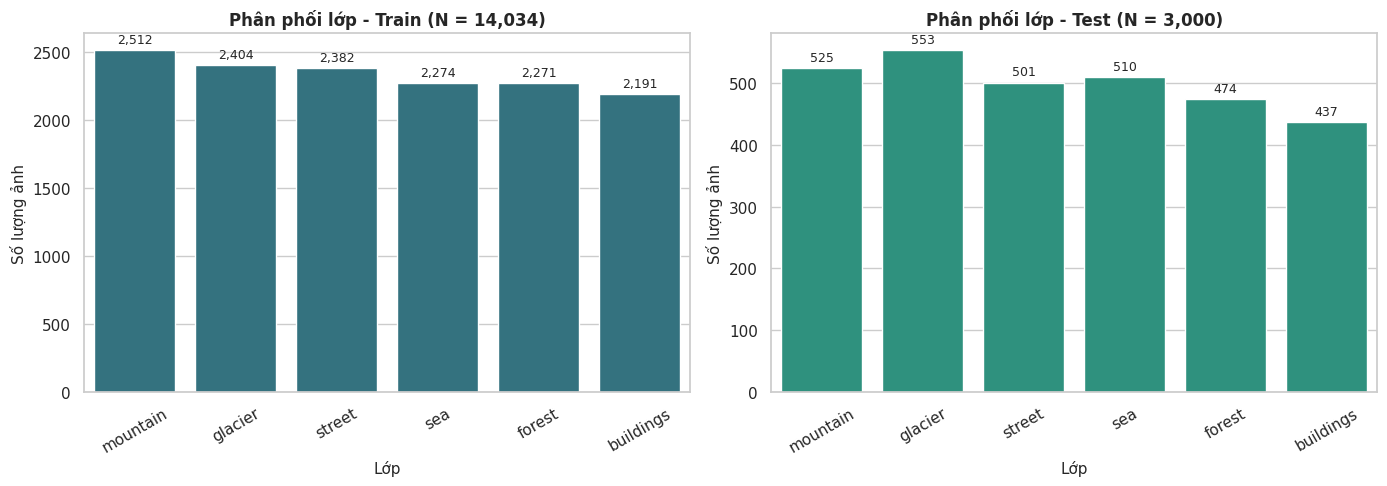
\includegraphics[width=0.86\linewidth]{image/c11_f0.png}
  \caption{Phân phối số lượng ảnh theo 6 lớp trên tập Train (14.034 ảnh) và Test (3.000 ảnh): các lớp tương đối cân bằng (14,57\% -- 18,43\%), không cần áp dụng kỹ thuật cân bằng lớp nhân tạo.}
  \label{fig:img_dist}
\end{figure}

Nhóm tách tập Train ban đầu theo tỷ lệ phân tầng (\textit{Stratified Split}) thành \textbf{Train (85\% -- 11.928 ảnh)} và \textbf{Validation (15\% -- 2.106 ảnh)}, giữ nguyên \textbf{Test (3.000 ảnh)} độc lập. Trực quan hóa bằng t-SNE trên 24 đặc trưng histogram màu RGB toàn cục (\Cref{fig:img_tsne}) cho thấy \textit{forest} tách biệt khá rõ nhờ sắc xanh lá, trong khi \textit{glacier} -- \textit{mountain} và \textit{buildings} -- \textit{street} chồng lấn mạnh do chia sẻ tông màu và cấu trúc nền.

\begin{figure}[H]
  \centering
  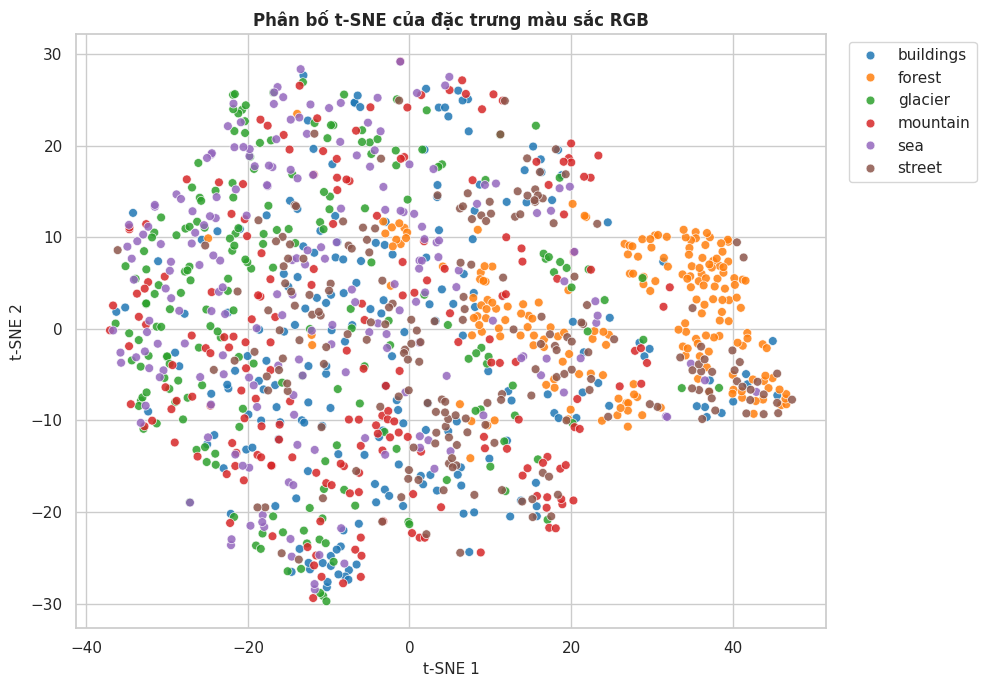
\includegraphics[width=0.84\linewidth]{image/c25_f0.png}
  \caption{Trực quan hóa t-SNE từ đặc trưng màu RGB toàn cục (1.200 mẫu): đặc trưng màu thủ công phân tách tốt \textit{forest}, nhưng chồng lấn nặng giữa \textit{mountain}--\textit{glacier} và \textit{buildings}--\textit{street}, chứng minh cần đặc trưng không gian sâu.}
  \label{fig:img_tsne}
\end{figure}

\subsection{Thiết kế thực nghiệm và Pipeline huấn luyện}
Nhóm sử dụng chuẩn \textit{Data Augmentation} trên tập Train (RandomResizedCrop/Resize, HorizontalFlip, ColorJitter nhẹ và chuẩn hóa theo thống kê ImageNet) với \texttt{batch\_size = 64} trên GPU Tesla T4. Bảy cấu hình mô hình thuộc 4 hệ quy chiếu được đối chiếu công bằng trên cùng tập Test 3.000 ảnh:
\begin{enumerate}[leftmargin=*]
  \item \textbf{Huấn luyện từ đầu (\textit{From Scratch}):} \texttt{SimpleBaselineCNN} (0,42M tham số, 10 epochs) và \texttt{ResNet-18 Scratch} (11,18M tham số, 12 epochs).
  \item \textbf{Pretrained Feature Extractor (\textit{Linear Probe}):} \texttt{ResNet-18} đóng băng backbone, chỉ huấn luyện lớp phân loại cuối (3.078 tham số, 5 epochs).
  \item \textbf{Pretrained Fine-tuning:} \texttt{ResNet-18} mở khóa \texttt{layer4+fc} (8,40M tham số, 6 epochs) và \texttt{ViT-B/16} (14,18M tham số huấn luyện / 85,80M tổng, 6 epochs).
  \item \textbf{Zero-shot Foundation Model:} \texttt{CLIP ViT-B/32} \cite{radford2021learning} (không huấn luyện, 0 tham số cập nhật) với cấu hình Basic và Prompt Ensemble.
\end{enumerate}

\subsection{Bảng đối chiếu Benchmark và Đánh đổi kỹ thuật}

\Cref{tab:img_benchmark} và \Cref{fig:img_benchmark} tổng hợp toàn diện độ chính xác, tốc độ suy luận và tài nguyên VRAM của cả 7 mô hình trên tập Test.

\begin{table}[H]
  \centering
  \caption{Bảng đối chiếu hiệu năng và chi phí kỹ thuật của 7 mô hình trên tập Test độc lập (3.000 ảnh).}
  \label{tab:img_benchmark}
  \resizebox{\linewidth}{!}{%
  \begin{tabular}{l l r r r r r r}
    \toprule
    \textbf{Mô hình} & \textbf{Phương pháp} & \textbf{Trainable} & \textbf{Train (s)} & \textbf{VRAM (MB)} & \textbf{Latency (ms)} & \textbf{Test Acc (\%)} & \textbf{Macro-F1 (\%)} \\
    \midrule
    ViT-B/16 (Fine-tune) & Vision Transformer & 14,18M & 1262,8 & 2276,6 & 11,20 & \textbf{94,87} & \textbf{94,98} \\
    ResNet-18 (Fine-tune) & Partial Fine-tune & 8,40M & 439,2 & 753,4 & 3,42 & 93,90 & 93,99 \\
    CLIP ViT-B/32 (Ensemble) & Zero-shot VLM & 0 & 0,0 & 1441,4 & 5,17 & 93,43 & 93,58 \\
    CLIP ViT-B/32 (Basic) & Zero-shot VLM & 0 & 0,0 & 1441,4 & 5,08 & 93,00 & 93,10 \\
    ResNet-18 (Linear Probe) & Frozen Backbone & 3.078 & 391,7 & 606,9 & 3,00 & 89,87 & 90,02 \\
    ResNet-18 (Scratch) & From Scratch & 11,18M & 577,9 & 909,3 & 2,02 & 89,40 & 89,50 \\
    SimpleBaselineCNN & From Scratch & 0,42M & 458,3 & 1048,2 & \textbf{1,76} & 85,80 & 85,87 \\
    \bottomrule
  \end{tabular}%
  }
\end{table}

\begin{figure}[H]
  \centering
  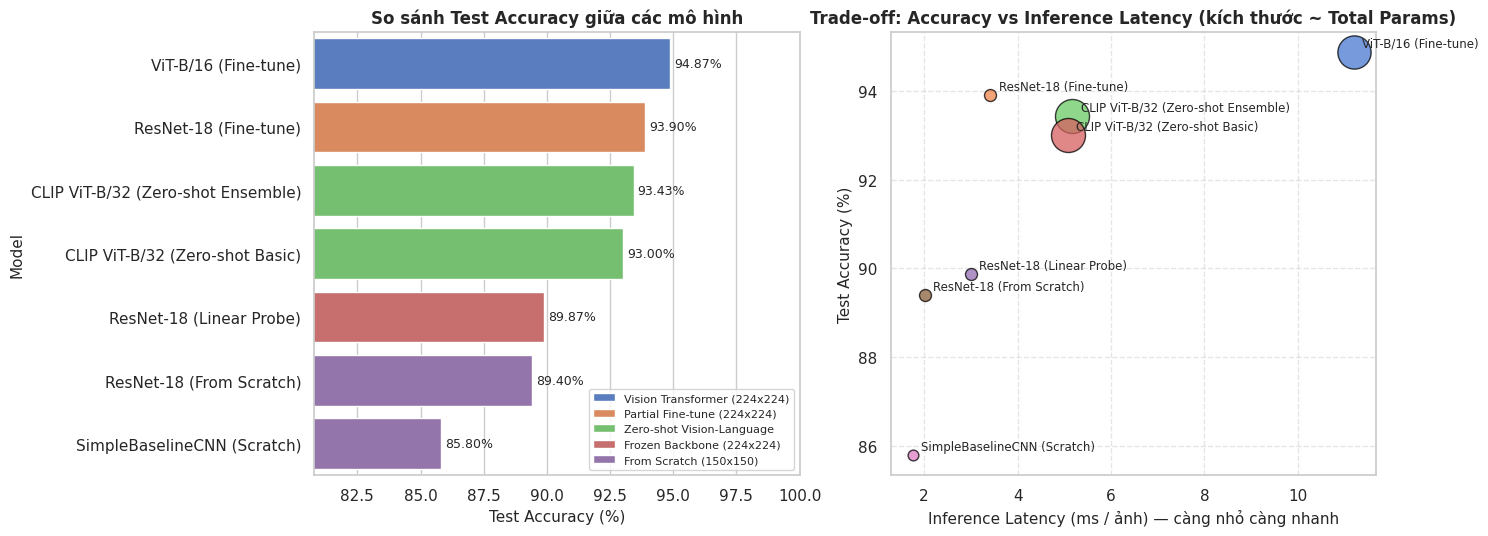
\includegraphics[width=0.90\linewidth]{image/c53_f0.png}
  \caption{Đối chiếu Test Accuracy, Macro-F1 và độ trễ suy luận giữa 7 mô hình: \textit{ViT-B/16 (Fine-tune)} đạt Accuracy cao nhất (94,87\%) nhưng tốn 11,20 ms/ảnh; \textit{ResNet-18 (Fine-tune)} cân bằng tối ưu nhất (93,90\% với chỉ 3,42 ms/ảnh và 753,4 MB VRAM).}
  \label{fig:img_benchmark}
\end{figure}

Từ kết quả thực nghiệm rút ra 3 nhận định cốt lõi:
\begin{itemize}[leftmargin=*]
  \item \textbf{Transfer Learning vượt trội From Scratch:} \textit{ResNet-18 (Fine-tune)} đạt 93,90\%, cao hơn +4,50 điểm \% so với \textit{ResNet-18 (Scratch)} (89,40\%) và +8,10 điểm \% so với \textit{SimpleBaselineCNN} (85,80\%), đồng thời hội tụ nhanh hơn (6 epochs vs 12 epochs).
  \item \textbf{Sức mạnh của Zero-shot CLIP:} Không cần bất kỳ mẫu huấn luyện nào, \textit{CLIP ViT-B/32 (Ensemble)} đạt tới \textbf{93,43\%}, vượt qua cả \textit{ResNet-18 Linear Probe} (89,87\%). Đặc biệt, trên 183 ca \textit{ResNet-18 (Fine-tune)} đoán sai, \textit{CLIP} đoán đúng lại tới \textbf{93/183 ca (50,8\%)} và \textit{ViT-B/16} đoán đúng lại \textbf{80/183 ca (43,7\%)}.
  \item \textbf{Đánh đổi chi phí -- hiệu năng:} \textit{ViT-B/16} đạt đỉnh 94,87\% nhưng có độ trễ gấp 3,27 lần và VRAM gấp 3,02 lần so với \textit{ResNet-18 (Fine-tune)}.
\end{itemize}

\subsection{Phân tích lỗi và Minh bạch hóa bằng Grad-CAM (XAI)}
Ma trận nhầm lẫn (\Cref{fig:img_cm}) và danh sách mẫu sai (\Cref{fig:img_errors}) xác nhận đúng dự báo từ bước EDA: lỗi của \textit{ResNet-18 (Fine-tune)} tập trung chủ yếu ở hai cặp lớp giao thoa tự nhiên là \textit{mountain} $\leftrightarrow$ \textit{glacier} (45 ca mountain nhầm thành glacier [8,57\%] và 39 ca ngược lại [7,05\%]) và \textit{street} $\leftrightarrow$ \textit{buildings} (31 ca street nhầm thành buildings [6,19\%] và 24 ca ngược lại [5,49\%]). Trong khi đó, \textit{forest} (F1 = 99,26\%) và \textit{sea} (F1 = 96,82\%) đạt độ chính xác gần như tuyệt đối.

\begin{figure}[H]
  \centering
  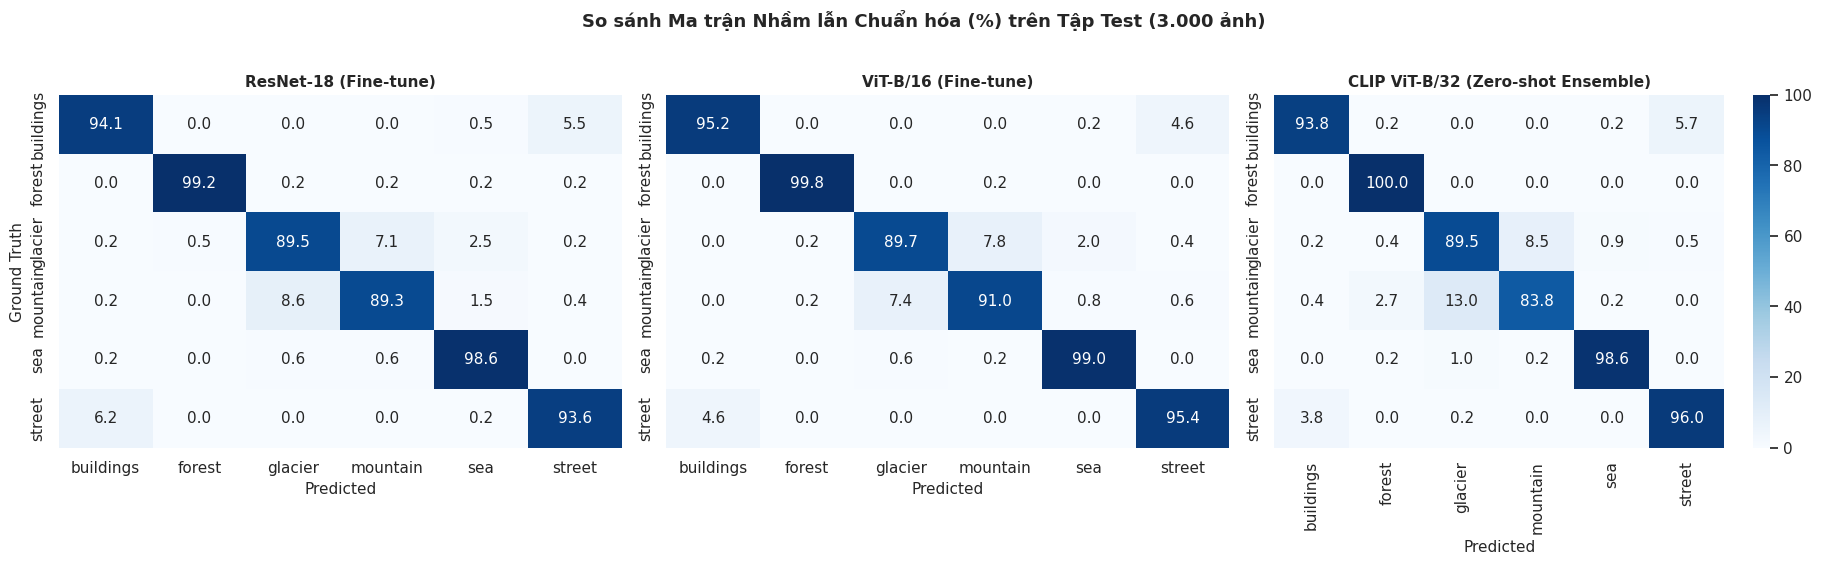
\includegraphics[width=0.90\linewidth]{image/c55_f0.png}
  \caption{Ma trận nhầm lẫn và F1-Score theo từng lớp: \textit{forest} đạt F1 99,26\% (ResNet-18 Fine-tune) và 99,68\% (ViT-B/16), trong khi phần lớn sai số nằm ở cặp \textit{mountain}--\textit{glacier} và \textit{buildings}--\textit{street}.}
  \label{fig:img_cm}
\end{figure}

\begin{figure}[H]
  \centering
  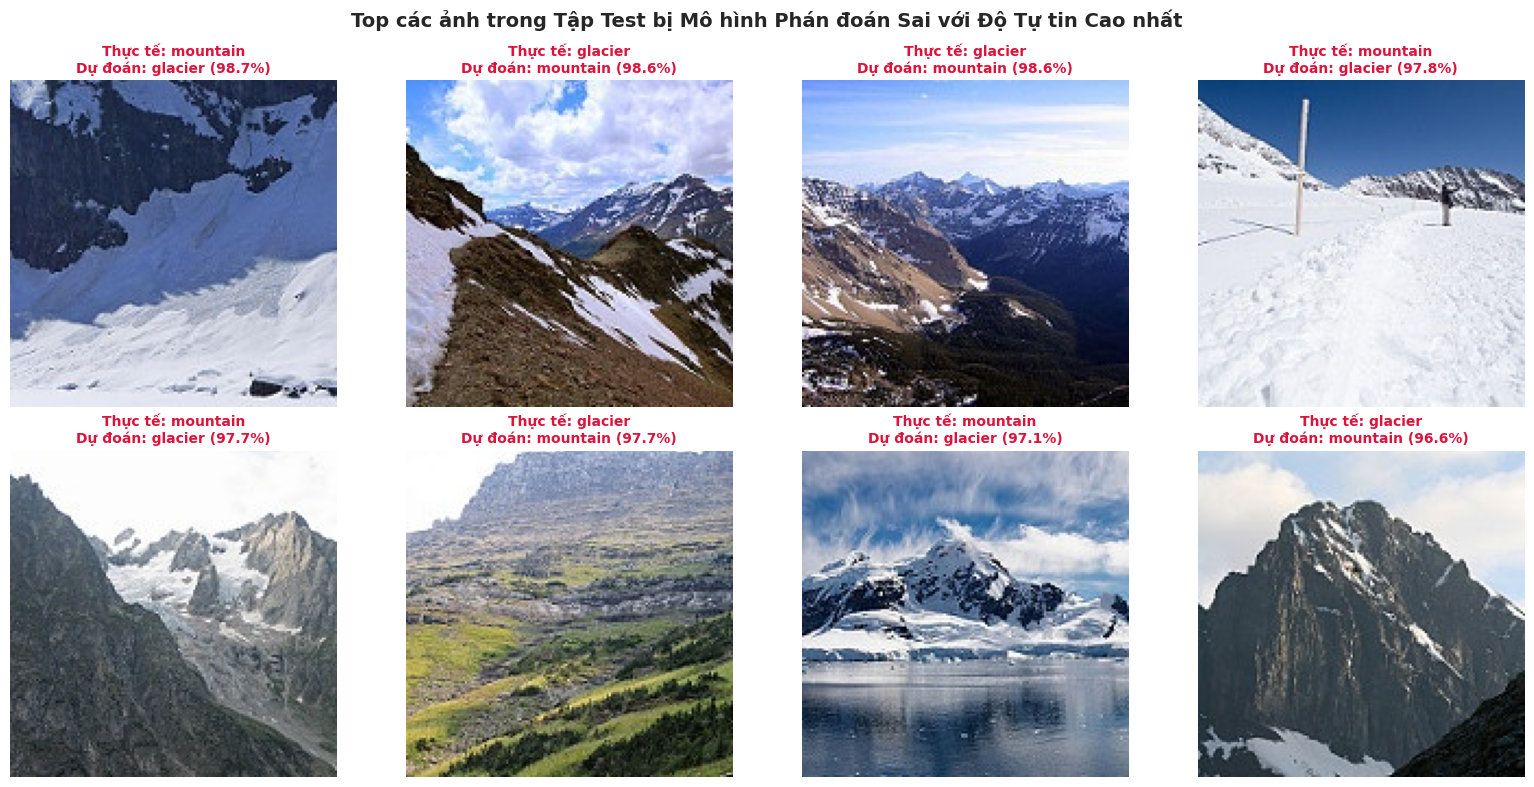
\includegraphics[width=0.88\linewidth]{image/c57_f0.png}
  \caption{Các mẫu dự đoán sai tiêu biểu của ResNet-18 (Fine-tune): nhiều ảnh chứa đồng thời cả tòa nhà và đường phố hoặc núi phủ tuyết, gây nhập nhằng ngay cả với mắt người.}
  \label{fig:img_errors}
\end{figure}

Sử dụng \textbf{Grad-CAM} (\Cref{fig:img_gradcam}) để giải thích vùng ảnh mô hình tập trung khi ra quyết định cho thấy: với các ca dự đoán đúng, \textit{ResNet-18 (Fine-tune)} định vị chính xác tán cây (\textit{forest}), mặt biển (\textit{sea}) hay mặt tiền công trình (\textit{buildings}); ngược lại ở các ca thất bại, mô hình bị phân tâm bởi vùng nền phụ (ví dụ bầu trời, sườn núi phủ tuyết hoặc dãy nhà ven đường).

\begin{figure}[H]
  \centering
  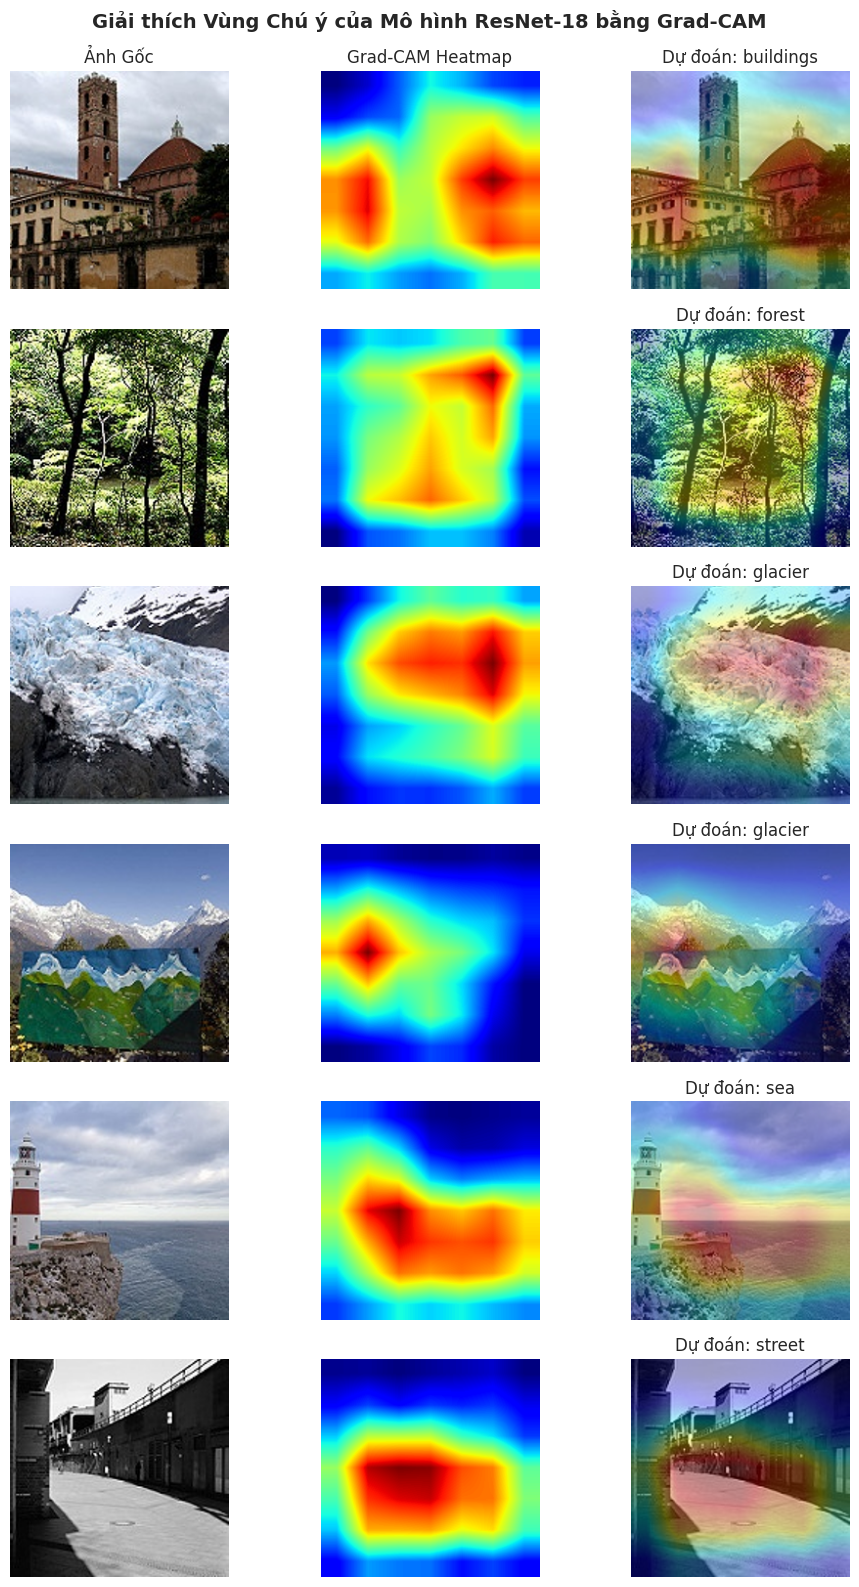
\includegraphics[width=0.88\linewidth]{image/c60_f0.png}
  \caption{Bản đồ nhiệt Grad-CAM minh họa cơ chế chú ý của ResNet-18 (Fine-tune): mô hình tập trung đúng vào đặc trưng đối tượng chính ở các mẫu dự đoán đúng và bị nhiễu nền ở các ca nhập nhằng.}
  \label{fig:img_gradcam}
\end{figure}

\section{Tổng kết chung}
\label{sec:conclusion}

Qua quá trình thực hiện bài tập lớn trên cả ba dạng dữ liệu (\textbf{Tabular}, \textbf{Text}, và \textbf{Image}), nhóm rút ra bốn bài học kỹ thuật trọng tâm:

\begin{enumerate}[leftmargin=*]
  \item \textbf{Kiểm tra toàn vẹn và chống rò rỉ dữ liệu quyết định tính tin cậy của mô hình:} Việc phát hiện missing ẩn (\texttt{-1}) và \textit{temporal shift} ở bài Tabular, cụm bài \textit{near-duplicate} và rò rỉ tên tác giả ở bài Text, hay tách tập phân tầng độc lập ở bài Image giúp tránh đánh giá lạc quan giả tạo (\textit{data leakage}).
  \item \textbf{EDA định lượng là kim chỉ nam cho tiền xử lý:} Mỗi bước tiền xử lý đều có thực nghiệm kiểm chứng — từ việc giữ cờ \texttt{\_flag} giúp giữ nguyên ROC-AUC $0,8986$ trên LightGBM, chuẩn hóa Unicode/bỏ dấu tiếng Việt và \texttt{StratifiedGroupKFold} cho LinearSVC đạt Macro-F1 $0,9668$, đến việc dùng Grad-CAM giải thích sai số trên cặp \textit{mountain}--\textit{glacier}.
  \item \textbf{Đối chiếu đa mô hình gắn với bài toán triển khai:} Không có mô hình tốt nhất tuyệt đối cho mọi ngữ cảnh. Ở bài toán ảnh, \textit{ViT-B/16 (Fine-tune)} đạt Accuracy cao nhất (94,87\%) nhưng \textit{ResNet-18 (Fine-tune)} lại tối ưu hơn cho hệ thống thời gian thực (93,90\% với độ trễ chỉ 3,42 ms/ảnh), còn \textit{CLIP Zero-shot} (93,43\%) chứng minh hiệu quả vượt trội khi thiếu dữ liệu gán nhãn.
  \item \textbf{Tính công bằng và giới hạn thực tế:} Trong bài toán tài chính nhạy cảm (\textit{Bank Account Fraud}), tối ưu hóa một ngưỡng duy nhất có thể gây bất công cho nhóm khách hàng $\ge 50$ tuổi ($\text{FPR} = 10,12\%$ vs $3,35\%$). Việc thiết lập ngưỡng theo nhóm giúp đưa tỷ lệ báo động nhầm về mức cân bằng ($\text{FPR ratio} = 1,014$), đồng thời chỉ ra sự cần thiết của kiểm định công bằng (\textit{Fairness auditing}) trước khi đưa mô hình vào vận hành.
\end{enumerate}


\clearpage
\bibliographystyle{plain}
\bibliography{refs/references.bib}

\end{document}
